\documentclass[12pt, a4paper]{report}
\usepackage{graphicx}
\usepackage{colortbl}
\usepackage[brazilian]{babel}
\usepackage[utf8x]{inputenc}
\usepackage{setspace}
\usepackage{hyperref}
\usepackage[small,bf]{caption}
\usepackage{amsmath, amssymb, pxfonts}
\usepackage{textcomp}
\usepackage{nomencl}
\makenomenclature
\usepackage{longtable}
\usepackage{tikz}
\usepackage{pgfplots}
\usepackage{mathrsfs}
\everymath{\displaystyle}
\usepackage[alf]{abntex2cite}
\usepackage{url}
\usepackage{emptypage}
\usepackage{fancyhdr}
\usepackage{lastpage}
\usepackage{nopageno}
\usepackage{indentfirst}
\usepackage{parskip}
\usepackage{titlesec}
\usepackage{listings}
\usepackage{subfig}
\usepackage{verbatim}
\usepackage{multirow}

%%%%%%%%%%%%%%%%%%%%%%%%%%%%%%%%%%%%%%%%%%%%%%%%%%%%%%%%%%%%%%%%%%%%
%%%
%%% Macros 
%%% Curso de Especialização em Sistemas Eletrônicos para Controle
%%% Faculdade SENAI Anchieta - São Paulo - SP
%%% José William Rodrigues Pereira 
%%% Outubro / 2015
%%%
%%%%%%%%%%%%%%%%%%%%%%%%%%%%%%%%%%%%%%%%%%%%%%%%%%%%%%%%%%%%%%%%%%%%

%%%------------------------------------ Dados
\def\autor#1{\gdef\autor{#1}}
\def\nome#1{\gdef\nome{#1}}
\def\ultimonome#1{\gdef\ultimonome{#1}}
\def\titulo#1{\gdef\titulo{#1}}
\def\subtitulo#1{\gdef\subtitulo{#1}}
\def\curso#1{\gdef\curso{#1}}
\def\instituicao#1{\gdef\instituicao{#1}}
\def\sigla#1{\gdef\sigla{#1}}
\def\unidadeacademica#1{\gdef\unidadeacademica{#1}}
\def\grau#1{\gdef\grau{#1}}
\def\tipodotrabalho#1{\gdef\tipodotrabalho{#1}}
\def\orientador#1{\gdef\orientador{#1}}
\def\torientador#1{\gdef\torientador{#1}}
\def\coorientador#1{\gdef\coorientador{#1}}
\def\tcoorientador#1{\gdef\tcoorientador{#1}}
\def\cidade#1{\gdef\cidade{#1}}
\def\ano#1{\gdef\ano{#1}}
\def\npaginas#1{\gdef\npaginas{#1}}
\def\CDU#1{\gdef\CDU{#1}}
\def\areas#1{\gdef\areas{#1}}
\def\examinadorum#1{\gdef\examinadorum{#1}}
\def\texaminadorum#1{\gdef\texaminadorum{#1}}
\def\examinadordois#1{\gdef\examinadordois{#1}}
\def\texaminadordois#1{\gdef\texaminadordois{#1}}
\def\data#1{\gdef\data{#1}}
\def\palavraschave#1{\gdef\palavraschave{#1}}
\def\keywords#1{\gdef\keywords{#1}}

%%%%------------------------------------ Configuração das Páginas
\newcommand{\configuramargens} %%% Define margens
{
  \usepackage[width=210.00mm, height=297.00mm, 
			  left=3.00cm,    right=2.00cm, 
			  top=3.00cm,     bottom=2.00cm] {geometry}
}

%%%------------------------------------ Fonte
%\renewcommand{\familydefault}{\sfdefault} % sans font
\renewcommand{\familydefault}{\rmdefault}  % roman font


%%%------------------------------------ Formatação de Capitulo
\titleformat{\chapter}
  {\Large\bfseries}
  {}
  {0pt}
  {\huge}

%%%------------------------------------ Capa
\newcommand{\capa}
{
  \begin{titlepage}
    \thispagestyle{empty}
    \begin{center}
      \textsc{\instituicao} 		\\[5.0cm]
%      \textsc{\unidadeacademica}	\\[0.0cm]
%      \textsc{Curso de \curso}		\\[4.0cm]
      \textsc{\autor}			\\[5.0cm]
      \textsc{\titulo}			\\[0.0cm]
      \textsc{\subtitulo}               \\[0.4cm]
      \vfill
      \textsc{\cidade}			\\[0.0cm]
      \textsc{\ano}			\\[0.0cm]
    \end{center}
  \end{titlepage}
}
%%%------------------------------------ Natureza
\newcommand{\natureza}
{
  \begin{flushright}
    \thispagestyle{empty}
    \begin{minipage}{0.54\textwidth}
    {
      \tipodotrabalho apresentada ao \instituicao 
      como requisito para 
      obtenção do grau de \grau em \curso
    } 				\\[0.4cm]
    Orientador:   \torientador    \orientador \\
%    Coorientador: \tcoorientador  \coorientador
    \end{minipage}
  \end{flushright}
}
%%%------------------------------------ Folha de Rosto
\newcommand{\folhaderosto}
{
  \begin{titlepage}
    \begin{center}
      \textsc{ }		\\[5.0cm]
      \textsc{\autor}		\\[5.0cm]
      \textsc{\titulo}		\\[0.0cm]
      \textsc{\subtitulo}       \\[4.0cm]
      \natureza
      \vfill
      \textsc{\cidade}		\\[0.0cm]
      \textsc{\ano}		\\[0.0cm]
    \end{center}
  \end{titlepage}
}
%%%------------------------------------ Ficha Catalográfica
\newcommand{\fichacatalografica}
{
  \begin{titlepage}
    \vfil\null
    \vfill
    \fbox
    {
      \begin{tabular}{p{13.0cm}}
        \ultimonome, \nome                      \\
        \titulo \subtitulo\ / \nome\ \ultimonome\ -  \ano \\
        \npaginas .p                \\
        \areas . I.Título. \\
        \hfill CDU \CDU
      \end{tabular} 
    }  
 \end{titlepage}
}
%%%------------------------------------ Folha de Aprovação
\newcommand{\folhadeaprovacao}
{
  \begin{titlepage}
    \thispagestyle{empty}
    \begin{center}
      \textsc{\autor}
      \vfill
      \textsc{ \titulo } \\
      \textsc{ \subtitulo }
      \vfill
    \end{center}
    \natureza
    \vfill
    \centering Aprovado pela banca examinadora em \data \\
    \vfill
    \begin{center}
      {\large\bfseries BANCA EXAMINADORA }\\
      \vfill
      \rule{9.0cm}{0.1mm} \\
      {\torientador \orientador  }\\
      {Orientador } \\
 %     \vfill
 %     \rule{9.0cm}{0.1mm} \\
 %     {\tcoorientador \coorientador} \\
 %     {Coorientador} \\
      \vfill
      \rule{9.0cm}{0.1mm} \\
      {\texaminadorum \examinadorum }\\
      \vfill
      \rule{9.0cm}{0.1mm} \\
      {\texaminadordois \examinadordois}
    \end{center}
  \end{titlepage}
}
%%%------------------------------------ Dedicatória
\newcommand{\dedicatoria}[1]
{
  \begin{titlepage}
  \thispagestyle{empty}
  \hspace{1cm}
  \vfill
  \begin{flushright}
    \begin{minipage}{0.6\textwidth}
    \textrm
    {
      \textit
      {
	#1
      }
    }    
    \end{minipage}
  \end{flushright}
  \end{titlepage}
}

%%%------------------------------------ Agradecimentos
\newcommand{\agradecimentos}[1]
{
  \begin{titlepage} 
    \thispagestyle{empty}
    \titlepage
    \begin{center}%
        \huge \textbf{Agradecimentos}
    \end{center}%
    \null
    \hspace{1cm} #1
    \endtitlepage
  \end{titlepage}
}

%%%------------------------------------ Epígrafe
\newcommand{\epigrafe}[1]
{
  \begin{titlepage}
    \thispagestyle{empty} 
    \hspace{1cm}
    \vfill
    \begin{flushright}
      \begin{minipage}{0.6\textwidth}
      \textrm
      {
        \textit
        {
	    #1
        }
      }    
      \end{minipage}
    \end{flushright}
  \end{titlepage}
}

%%%------------------------------------ Resumo
\newcommand{\resumo}[1]
{
  \begin{titlepage} 
    \titlepage  
    \thispagestyle{empty}
    \begin{center}%
        \huge \textbf{Resumo}
    \end{center}%
    \null
    #1

    \textbf{\\PALAVRAS-CHAVE:} \palavraschave
    \endtitlepage
  \end{titlepage}
}
%-------------------------------------- Abstract
\newcommand{\resumolinguaestrangeira}[1]
{
  \begin{titlepage} 
    \titlepage
    \thispagestyle{empty}  
    \begin{center}%
        \huge \textbf{Abstract}
    \end{center}%
    \null  
    \hspace{1cm} 
    #1

    \textbf{\\KEYWORDS:} \keywords
    \endtitlepage
  \end{titlepage}
}
%-------------------------------------- Sumário
\newcommand{\sumario}
{
    \tableofcontents
    \thispagestyle{empty}
}
%-------------------------------------- Lista de figuras
\newcommand{\listadefiguras}
{
  \listoffigures
  \thispagestyle{empty}
}
%-------------------------------------- Lista de tabelas
\newcommand{\listadetabelas}
{
  \listoftables
  \thispagestyle{empty}
}

%-------------------------------------- Lista de abreviaturas e siglas
\newcommand{\abreviatura}[2]
{
  \nomenclature{#1}{#2}
  #1
}
\newcommand{\listadeabreviaturasesiglas}
{
  \renewcommand{\nomname}{Lista de abreviaturas e siglas}
  \printnomenclature[5em]
  \thispagestyle{empty}	
}
%%%------------------------------------ Citação
\newcommand{\citacao}[1]
{
  \begin{flushright}
    \begin{minipage}{12cm}
      \footnotesize #1
    \end{minipage}
    \vspace{12pt}
  \end{flushright}
}

%--------------------------------------
%--------------------------------------


%--------------------------------------
%-------------- Estilo do Codigo Fonte
\definecolor{verde}{rgb}{0.25,0.5,0.35}
\definecolor{jpurple}{rgb}{0.5,0,0.36}

\lstset{
  language=C,
  basicstyle=\ttfamily\small,
  keywordstyle=\color{blue},
  stringstyle=\color{verde},
  commentstyle=\color{red},
  extendedchars=true,
  showspaces=false,
  showstringspaces=false,
  numbers=left,
  numberstyle=\small,
  breaklines=true,
  backgroundcolor=\color{green!10},
  breakautoindent=true,
  captionpos=b,
  xleftmargin=0pt,
}

%--------------------------------------:w








%%%----------------------------------- Declarações
\autor{JOSÉ WILLIAM RODRIGUES PEREIRA}
\nome{José William Rodrigues }
\ultimonome{Pereira}
\titulo{ CONTROLE DE SISTEMA DINÂMICO UTILIZANDO LÓGICA PARACONSISTENTE ANOTADA DE ANOTAÇÃO COM DOIS VALORES (LPA2v)
%ESTUDO DA MALHA DE CONTROLE APLICANDO LÓGICA PARACONSISTENTE ANOTADA DE ANOTAÇÃO COM DOIS VALORES (LPA2v)
}
\subtitulo{ }
\curso{Automação e Controle de Processos }
\instituicao{Instituto Federal de Educação, Ciência e Tecnologia de São Paulo }
\sigla{IFSP}
\unidadeacademica{Pós-Graduação Stricto Sensu }
\grau{Mestre }
\tipodotrabalho{Qualificação } 
\orientador{Tarcisio Fernandes Leão }
\torientador{Profº Dr. }
\coorientador{ }
\tcoorientador{  }
\cidade{São Paulo}
\ano{2017}
\npaginas{\pageref{LastPage}}
\CDU{xxx.yy}
\areas{	1.Técnicas de Controle 
	2.Lógica Paraconsistente
	3.Controle Não-Convencional}
\examinadorum{ Alexandre Brincalepe Campo}
\texaminadorum{Profº Dr.}
\examinadordois{Cláudio Rodrigo Torres}
\texaminadordois{Profº Dr. }
\data{dd/mm/aaaa}
\palavraschave{Controle Não Convencional; Lógica Paraconsistente; Técnicas de Controle }
\keywords{ Unconventional control; Paraconsistent logic; Control Techniques; }


%%%%%%%%%%%%%%%%%%%%%%%%%%%%%%%%%%%%%%%%
%%%% Inicio do documento
%%%%%%%%%%%%%%%%%%%%%%%%%%%%%%%%%%%%%%%%
\configuramargens


\setlength{\parindent}{1cm}
\setlength{\parskip}{12pt}



\begin{document}
\capa

\folhaderosto
%\fichacatalografica
\folhadeaprovacao

%\dedicatoria{      Dedico este trabalho à minha família, 
      pela paciência;
      aos amigos de curso e professores, 
      pelo companheirismo e dedicação;
      a todos que em algum momento compartilharam 
      ideias, palavras de incentivo e carinho;
      A todos os amantes do saber.
}
%\agradecimentos{À minha família e à minha esposa Fernanda, 
que além de apoio incondicional souberam 
compreender todo o esforço e dedicação destinados a este trabalho.

Ao Profº Dr. Tarcisio Fernandes Leão 
por acreditar no potencial deste trabalho,
pela orientação ativa e sempre bem humorada, 
pela dedicação e apoio tanto em sala quanto em conversas informais, 
desde sempre. 

Ao Profº Me. Vander Célio Nunes por apresentar e ensinar a 
Lógica Paraconsistente Anotada Evidencial $E\tau$ , 
pela dedicação e amor ao ensino.

Ao Instituto Federal de Educação Ciência e Tecnologia de São Paulo, 
em todo seu corpo docente de qualidade reconhecida, 
que foram e ainda são um referencial e um objetivo 
de formação profissional e de excelência nos diversos ramos 
do conhecimento educacional, científico e tecnológico, 
tanto na graduação quanto no programa de mestrado. 


À todos os colegas que fizeram parte desta jornada algo muito agradável, 
mostrando as individualidades e as potencialidades, 
ampliando a noção de respeito, parceria e amizade. 

 
}
%\epigrafe{{"Pense em nós como uma espécie de símbolo.
  Somos o sonho que a humanidade cria para dar sentido às sombras da
  caverna.
  Muito bem, agora vá em frente."
\\
  (Deuses Americanos)
\\
\\
\textbf{ Neil Gaiman } 
}


%  "Não é o pescado que você leva para casa no fim do dia.
%  É a paz de espírito."


%{"... Reze e trabalhe, fazendo de conta que esta vida é um dia de capina 
%com sol quente, que às vezes custa muito a passar, mas sempre passa. 
%E você ainda pode ter muito pedaço bom de alegria... 
%Cada um tem a sua hora e a sua vez: você há de ter a sua." (Sagarana)
%}
%{
%\\
%\\
%\textbf{ João Guimarães Rosa } 
%}
}
\resumo{%CONTEXTO: Identifica a grande area de pesquisa e sua importancia;

%LACUNA: (however:contudo, all do:todos fazem) O que precisa ser estudado nesse campo e ainda precisa ser entendido, exclarecido. Local aonde o trabalho está inserido;

%PRÓPOSITO: (this paper describes...)o que foi feito e principal objetivo do artigo;

%METODOLOGIA: Maneira geral falar dos métodos

%RESULTADOS: IMPORTANTÍSSIMO!!! Principal achado, resultado de forma bastante clara;

%CONCLUSOES: Mostrar como que os resutados contribuem para o avanço da grande aréa.

% Propósito
O objetivo deste estudo é mostrar uma implementação não convencional
de um controle em malha fechada utilizando a Lógica Paraconsistente
Anotada Evidencial $E\tau$ (LPA$E\tau$),
de forma a atender requisitos específicos de desempenho em um sistema físico proposto.
Sistemas de Controle são amplamente utilizados no setor industrial e
buscam uma maior eficiência de tempo e energia, mantendo uma qualidade
dos processos e do sistema controlado.
% Lacuna
O desenvolvimento de técnicas classificadas como Inteligência
Artificial fez surgirem outras opções para o controle de sistemas,
contudo ainda há escassez de implementações e testes usando técnicas alternativas.
% Metodologia
Para tanto é realizado um levantamento do modelo matemático desse
sistema físico, que é utilizado como referência para a implementação de um
controle clássico, com um controlador PI, bem como a definição dos
requisitos de desempenho do sistema, que norteiam a implementação
proposta utilizando a LPA$E\tau$, possibilitando assim a sua validação
por comparação entre os resultados dos controladores. 
% Resultados
Para o sistema testado,
os resultados entre os controladores
PI e LPA$E\tau$ foram equivalentes,
com ligeira vantagem a depender do
requisito de desempenho utilizado como referência.
Os resultados ainda mostraram algumas
possibilidades para futuras melhorias,
que se direcionam para plantas mais complexas,
como sistemas de segunda ordem,
e ainda permitem trabalhar com sistemas
sem a necessidade de conhecê-lo para controlá-lo,
adaptando seus parâmetros à ocasião
após algumas rodadas de aprendizado.
%Conclusão		
Os estudos e os resultados mostram um grande potencial para a
implementação e exploração da LPA$E\tau$ em sistemas de controle, de forma
semelhante as técnicas mais difundidas como uma Lógica Fuzzy, Redes
Neurais, Controle Adaptativo, Algorítmo Evolutivo, Inteligência
Artificial e Aprendizagem de máquina, inclusive
utilizando-as como suporte de geração de parâmetros de controle.


}
\resumolinguaestrangeira{%CONTEXT: Identifies the large area of ​​research and its importance;

% LACUNA: (however: however, all do: all do)
%What needs to be studied in this field and still needs to be
%understood, clarified.
%Place where the work is inserted;

% PRÓPOSITO: (this paper describes ...) what was done and main objective of the article;

% METHODOLOGY: General way of speaking of methods

% RESULTS: IMPORTANT! Main finding, result quite clear;

% CONCLUSIONS: Show how the results contribute to the advancement of the great area.

Control systems are widely used in the industrial sector and
seek efficiency of time and energy,
while maintaining a quality of processes and the controlled system.

% Purpose
The objective of this study is to show an unconventional implementation
of a closed-loop control using the Paraconsistent 
Annotated Logic Evidential $E\tau$ (PAL $E\tau$)
in order to meet specific performance requirements in a proposed physical system.

% Methodology
For this purpose a survey of the mathematical model of this
physical system, which is used as a reference for the implementation of a
with a PI controller,
as well as system performance requirements,
which guide the implementation of roposing to use PAL $E\tau$,
thus enabling its validation by comparison between the results of the controllers.

% Gap
The development of techniques classified as Intelligence
Artificial has given rise to other options for the control of systems,
however there is still a shortage of implementations and tests using alternative techniques.

% Results
For the system tested, the results between PI controllers and
PAL$E\tau$ were equivalent, with the rise time as
highlight, because for the tolerance window of $5\%$,
value was reached at $ t = 2.5s $ with the PI controller and 
$ t < 1.25s$ with the PAL$E\tau$ driver. 
The results still showed some
possibilities for future improvements, which
more complex systems, such as second-order systems, and
systems without the need to know
control it, adapting its parameters to the occasion after some
learning rounds.

%Conclusion
Initial studies and results show great potential for
implementation and exploitation of PAL$E\tau$ in control systems, in a
similar to the most widespread techniques such as a Fuzzy Logic, Networks
Neural Networks, Adaptive Control, Evolutionary Algorithm, Intelligence
Artificial and Machine Learning, including
using them as support for generation of control parameters.
}
\listadefiguras
%\listadetabelas
%\listadeabreviaturasesiglas

%\chapter*{Lista de símbolos}
%\thispagestyle{empty}
\begin{longtable}[l]{p{50pt} p{300pt}}
  $\mathscr{L} $ & Operador da Transformada de Laplace \\ \\
  $\mathscr{L}^{-1}$ & Operador da Transformada Inversa de Laplace\\ \\
  $s$ & Variável complexa de Laplace\\ \\
  $a$ & Polo da função \\ \\
  $c$ & Número real constante\\ \\
  $K$ & Constante de proporcionalidade\\ \\
  $e$ & Número de Euler, função exponencial\\ \\
  $\tau$ & Intervalo de tempo que uma curva de 1º grau alcança 64\% do valor de regime\\ \\
  $\rightarrow$ & Em lógica: Implica; Em cálculo: tende a\\ \\
  $\forall$ & Para todo\\ \\
  $\neg$ & Negação\\ \\
  $\vee$ & Disjunção\\ \\
  $\wedge$ & Conjunção\\ \\
  $\mu $ & grau de evidência favorável \\ \\
  $\lambda $ & grau de evidência desfavorável \\ \\
  $\Re$ & Conjunto dos números reais\\ \\
  $\in$ & Pertence\\ \\
  $\subset$ & Está contido em\\ \\
  $V$ & Verdadeiro\\ \\
  $F$ & Falso\\ \\
  $\top$ & Contradição\\ \\
  $\bot$ & Paracompleto\\ \\
  $\sim$ & Negação\\ \\
  $\leftrightarrow$ & Transposta\\ \\
\end{longtable}




\sumario

%\singlespacing 	% espaçamento simples
\onehalfspacing		% espaçamento de 1,5
%\doublespacing		% espaçamento duplo

\pagestyle{myheadings}
%\pagestyle{fancy}

%\fancyhf{}
%\lhead{\pageref{LastPage}}
%\rhead{\thepage}

\setcounter{page}{6}
\chapter[Introdução]{1. Introdução}
%%%Objetivo ou Finalidade: preocupação em distinguir a característica comum ou as leis gerais que regem determinados eventos.

Tendo em vista que estudos de novas formas de lógicas não clássicas estão em curso, a lógica paraconsistente surge como uma promissora ferramenta para tomada de decisão em diversos campos de aplicação como a robótica, automação industrial, inteligência artificial, logística, controle, entre outras\cite{JoaoInacio}.
 
Segundo o Dr. \citeauthor{DecioKrause}(\citeyear{DecioKrause}), professor e pesquisador do departamento de Filosofia da Universidade Federal de Santa Catarina: "Alguns dos campos mais férteis de aplicação dessas lógicas têm sido a ciência da computação, a engenharia e a medicina." e cita ainda que:
\begin{citacao}{
 "... na inteligência artificial essas lógicas foram usadas a partir da década de 1980 por H. Blair e V. S. Subrahmanian, da Universidade de Siracusa, Estados Unidos, e colaboradores, na elaboração de sistemas para serem utilizados especialmente em medicina." 
}
\end{citacao}

A Lógica Clássica, que utiliza um modelo lógico binário, foi de forma muito natural adaptado ao funcionamento dos transistores utilizados como chave liga/desliga, e este funcionamento embasou toda a tecnologia digital que vemos hoje em dia, baseada em princípios bem definidos e reais. Assim, surge a indagação sobre a utilização de Lógicas Paraconsistentes aplicadas ao mundo real como cita \citeauthor{JISF2011}(\citeyear{JISF2011}):

\begin{citacao}{
Dentro desta percepção, surge a ideia da possibilidade real de um Sistema Lógico Paraconsistente que, assim como na lógica clássica, é um conjunto de axiomas e regras de inferência que objetivam representar formalmente raciocínio válido. Sendo assim, o Sistema Lógico Paraconsistente pode ser representado através de um algoritmo que tem sua utilização como o núcleo de um programa computacional com aplicações diretas em sistemas de Inteligência Artificial.
}
\end{citacao}



Algumas das Lógicas Paraconsistentes ainda não tiveram  uma abordagem prática de sua implementação, ou ainda, tais abordagens são muito escassas, seja com dispositivos simples ou com os mais complexos. 

Visando uma melhor compreensão da Lógica Paraconsistente, e vislumbrando sua utilização em controle de sistemas dinâmicos utilizando um ramo denominado Lógica Paraconsistente Anotada de Anotação com dois valores (LPA2v), pressupõe-se um estudo de uma aplicação inicial como forma de desbravar uma nova possibilidade da utilização de um algoritmo que vem sendo aplicado com sucesso em Inteligência Artificial no segmento de Controle.






%%%%%%%%%%%%%%%%%%%%%%%%%%%%%%%%%%%%%%%%%%%%%%%%%%%%%%%%%%%%
\section{Hipótese e Relevância do Trabalho}
%%%%%%%%%%%%%%%%%%%%%%%%%%%%%%%%%%%%%%%%%%%%%%%%%%%%%%%%%%%%
A Lógica Paraconsistente Anotada de anotação com dois valores (LPA2v) pode ser utilizada para o controle de sistemas dinâmicos, hipótese esta que confirmada pode elevar ainda mais a sua relevância e elencar mais uma alternativa para aplicações técnicas e científicas. 

A lógica paraconsistente vem ganhando relevância e adeptos principalmente a partir do final da década de 90 do século XX, quando houve o Primeiro Congresso Mundial sobre Paraconsistência em Gent na Bélgica em 1997, no ano 2000 o segundo congresso realizado em São Sebastião, São Paulo e o terceiro em Toulouse, França em julho de 2003, atraindo cada vez mais pesquisadores interessados de diversos centros de pesquisa do mundo \cite{DecioKrause}. 

Em meados de setembro de 2016, aconteceu o pela primeira vez no Brasil a XVI Conferência Internacional de Lógica: \texttt{Tendências da Lógica} (\emph{Trends In Logic XVI - Studia Logica International Conference}) \cite{trendsinlogic}, realizada pelo Centro de Lógica, Epistemologia e História da Ciência (CLE) da Universidade Estadual de Campinas, que reuniu estudiosos brasileiros e de diversos países com trabalhos e apresentações sob o tema: Consistência, Contradição, Paraconsistência e Racioncínio (\emph{Consistency, Contradiction, Paraconsistency, and Reasoning}).

Atualmente as pesquisas estão focadas no estudo da aplicação da Lógica Paraconsistente, e ganhar espaço no universo técnico e científico, contribuindo com uma nova e eficiente forma de trabalho.





%%%%%%%%%%%%%%%%%%%%%%%%%%%%%%%%%%%%%%%%%%%%%%%%%%%%%%%%%%%%
\section{Objetivo Geral}
%%%%%%%%%%%%%%%%%%%%%%%%%%%%%%%%%%%%%%%%%%%%%%%%%%%%%%%%%%%%
%Objeto, subdividido em:
%Material: aquilo que pretende estudar, analisar, interpretar ou verificar de modo geral.
Estudar a LPA2v e desenvolver um algoritmo que possa ser embarcado para atuar no controle dinâmico de um sistema físico.




%%%%%%%%%%%%%%%%%%%%%%%%%%%%%%%%%%%%%%%%%%%%%%%%%%%%%%%%%%%%
\section{Objetivos Específicos}
%%%%%%%%%%%%%%%%%%%%%%%%%%%%%%%%%%%%%%%%%%%%%%%%%%%%%%%%%%%%
%Formal:enfoque especial, 
%	em face de diversas ciências que possuem o mesmo objetivo material.


Realizar a construção de um sistema físico para o controle de velocidade em um motor DC, de modo a utilizá-lo para a realização dos ensaios.

Implementar o algorítmo da LPA2v proposto na literatura de referência, codificando-o e criando uma biblioteca para sua utilização junto ao sistema físico.

Desenvolver a malha de controle do sistema físico proposto utilizando o algorítmo da LPA2v.




%%%%%%%%%%%%%%%%%%%%%%%%%%%%%%%%%%%%%%%%%%%%%%%%%%%%%%%%%%%%
\section{Justificativa}
%%%%%%%%%%%%%%%%%%%%%%%%%%%%%%%%%%%%%%%%%%%%%%%%%%%%%%%%%%%%

%Função:aperfeiçoamento, 
%	através de crescente acervo de conhecimento, 
%	da relação do homem com o seu mundo.


A função primordial do presente trabalho é realizar uma análise da implementação de uma lógica não-convencional, 
contribuindo para a ampliação do conhecimento em uma nova forma de lidar com o mundo e
gerar aplicações em uma área ainda pouco explorada pela LPA2v, o controle de sistemas. 


A visão aristotélica cunhou a forma lógica de lidar com o mundo, 
estabelecendo regras que permearam a história até o presente momento,
mas que, no século XX foram questionadas, procurando-se novas formas e ferramentas para tratar de questões que fogem das regras vigentes. 
A Lógica Paraconsistente é uma das ferramentas que permite o tratamento de contradições e incertezas,
que estão além dos limites da lógica clássica.

A LPA2v é a uma vertente da Lógica Paraconsistente que vem sendo explorada para finalidades práticas, 
tais como o reconhecimento de padrões em banco de dados, tomada de decisão e tratamento de incertezas em sistemas robóticos e logísticos, 
mas todas as áreas com uma abordagem ligada à Inteligência Artificial ou ao controle discreto do processo, 
ainda há escassez de trabalhos no controle contínuo de sistemas dinâmicos. 


A análise da implementação da LPA2v no universo das lógicas não-convencionais implica em possibilitar uma nova forma de controle de sistemas, 
sua definição permite um embasamento para criar novas possibilidades de seu uso,
e ajudar a sedimentar a nova ferramenta no meio acadêmico. 



%%%%%%%%%%%%%%%%%%%%%%%%%%%%%%%%%%%%%%%%%%%%%%%%%%%%%%%%%%%%
%\section{Limitações da pesquisa}
%%%%%%%%%%%%%%%%%%%%%%%%%%%%%%%%%%%%%%%%%%%%%%%%%%%%%%%%%%%%

%%% Não colocar o elemento TEMPO! 
%%% Colocar até onde vai a pesquisa e o que ela não abordará.

%Este estudo limitar-se-á ao estudo da LPA2v, e possivelmente uma pequena Rede de Análise Paraconsistente, voltado à Inteligência Artificial, mas sempre com o objetivo de realizar o controle dinâmico do sistema proposto.

%Não faz parte a abordagem do modo clássico de controle PID, Avanço de Fase, ou mesmo Controle Moderno, assim como a abordagem e especificações do controlador ou mesmo da linguagem utilizada para a montagem do protótipo.




\chapter[Revisão Bibliográfica]{2. Revisão Bibliográfica}
A modificação, de forma controlada, no comportamento de um sistema, 
garantindo uma maior eficiência é o objetivo do controle de sistemas,
que é estudado desde os antigos, mas que obteve grande relevância na necessidade trazida com a revolução industrial, 
e hoje conta com o seu segmento específico da engenharia, com diversos trabalhos nessa área e uma infinidade de aplicações. 
 

A principal tarefa de um engenheiro é, segundo \citeauthor{dorf2011modern}(\citeyear{dorf2011modern}), 
"o processo de concepção ou invenção de formas, partes e detalhes de um sistema para alcançar um propósito específico", 
processo este que soma a grande capacidade de análise e a criatividade para atender as demandas da função, 
como é o caso de projeto em engenharia no segmento de Sistemas de Controle, 
cujo objetivo é obter a configuração, as especificações e a identificação de processos para atender uma necessidade real. 


Uma concepção semelhante é trazida por \citeauthor{nise2009engenharia}(\citeyear{nise2009engenharia}) onde "Um sistema de controle consiste em subsistemas e processos(ou plantas) construídos com o objetivo de se obter uma saída desejada com desempenho desejado para uma entrada específica fornecida".


Os sistemas de controle atuam basicamente gerando respostas específicas para estímulos específicos de forma controlada e automática, 
trazendo vantagens nas aplicações em diversas áreas, tais como, 
na movimentação de grandes equipamentos com precisão, 
em locais remotos ou perigosos, 
na compensação de perturbações, 
manipulando os dados de forma conveniente.





%%%%%%%%%%%%%%%%%%%%%%%%%%%%%%%%%%%%%%%%%%%%%%%%%%%%%%%%%%%%
\section{Diagrama de Blocos}
%%%%%%%%%%%%%%%%%%%%%%%%%%%%%%%%%%%%%%%%%%%%%%%%%%%%%%%%%%%%



Os sistemas de controle são geralmente representados através de diagramas de blocos ou fluxo de sinais, 
como na Figura \ref{fig:processo}, 
convenientes ao seu desenvolvimento e análise. 
É composto por uma caixa representando o sistema a ser controlado, 
setas no sentido da caixa representando as entradas do processo e setas no sentido para fora da caixa para indicar a saída do sistema.


Em um sistema real podem haver muitas variáveis de entrada e de saída, 
mas a abordagem clássica de controle isola apenas uma das variáveis de entrada e uma de saída, 
ficando o sistema conhecido pela sigla em inglês SISO (\emph{Single In Single Out} - Única Entrada e Única Saída).


\begin{figure}[!htb]
\centering
\caption{ Diagrama de blocos de sistema de controle}
\begin{tikzpicture}[scale=1]
%\draw [lightgray](0,0) grid (9,2);
\draw (0,1) -- (3,1);
\draw [black, thick](3,0) rectangle (6, 2) ; 
\draw (6,1) -- (9,1);
\draw [fill](3,1) -- (2.8, 1.1) -- (2.8,0.9) -- (3,1);
\draw [fill](9,1) -- (8.8, 1.1) -- (8.8,0.9) -- (9,1);
\node at (4.5, 1){Sistema};
\node [above] at (1.5,1){Valor de};
\node [below] at (1.5,1){Referência};
\node [above] at (7.5,1){Variável};
\node [below] at (7.5,1){Controlada};
\end{tikzpicture}
\label{fig:processo}

{\small Fonte: \cite{Ogata} }
\end{figure}


O diagrama de blocos mostrado na Figura \ref{fig:processo} é uma simplificação ao máximo de um sistema de controle, 
contém apenas o bloco representando o sistema, 
uma entrada, para o valor de referência, 
e uma saída com o valor da variável controlada.


Em \citeauthor{Ogata}(\citeyear{Ogata}) % - Capítulo 3.3 - 
são encontradas definições, 
comentários sobre vantagens, 
aplicações e procedimento para construção de Diagramas de blocos, 
assim como a representação de sistemas em malha aberta, 
malha fechada, 
perturbações, 
técnicas e regras da álgebra de blocos.





%%%%%%%%%%%%%%%%%%%%%%%%%%%%%%%%%%%%%%%%%%%%%%%%%%%%%%%%%%%
\section{Ação de Controle}
%%%%%%%%%%%%%%%%%%%%%%%%%%%%%%%%%%%%%%%%%%%%%%%%%%%%%%%%%%%



A ação de controle é a forma como se busca atender os chamados requisitos de desempenho do sistema, 
que de um modo geral se efetuam através de modificações das características da relação entrada/saída para se obter os valores desejados dessa relação, 
ou ainda ajustar o comportamento da saída para uma dada entrada específica.


Os principais e mais comuns requisitos de desempenho dos sistemas são associados a velocidade de resposta, 
presença ou não de oscilações na estabilização e 
a exatidão da resposta do sistema em relação ao valor desejado, 
chamada de erro de regime estacionário.


O erro de regime estacionário, mostrada na Figura \ref{fig:funcaoResposta}, 
é uma medida que vai tender a zero em sistemas ideais, 
mas que na realidade não alcança o valor zero, 
assim assume-se um valor aceitável, 
5\% do valor da resposta desejada para sistemas não críticos e 
2\% para sistemas de maior grau de criticidade, 
para assumir que o sistema entrou em estabilidade, 
e a resposta real é aceita como tendo atingido o valor de resposta desejada. 



\begin{figure}[!htb]
\centering
\caption{Gráfico da função Resposta}
\begin{tikzpicture}[scale=1.00]
%\draw [lightgray, dashed](0,0) grid (8.8,5.8);

\draw [->] (0,0) -- (9,0); 
\draw [fill] (0,6.2) -- (-0.1, 5.8) -- (0.1,5.8) -- (0,6.2);

\draw [->] (0,0) -- (0,6);
\draw [fill] (9.2,0) -- (8.8,0.1) -- (8.8,-0.1)--(9.2,0.0);

\draw [purple, ->] (7.5,4.0) -- (7.5,4.6); 
\draw [purple, fill] (7.5,4.8) -- (7.4,4.5) -- (7.6,4.5)--(7.5,4.8);

\draw [purple, ->] (7.5,6.0) -- (7.5,5.2); 
\draw [purple, fill] (7.5,5.0) -- (7.4,5.3) -- (7.6,5.3)--(7.5,5.0);

\node at (9.0,-0.5) {$t$};
\node at (0.2,6.5) {$r(t)$};

\draw [blue, ultra thick] (0.0,5.0) -- (9.0,5.0);
\draw [blue, ultra thick] (0.0,0.0) -- (0.0,5.0);

\draw [red, ultra thick] (0,0) to [out=85, in=180] (6,4.8);

\draw [purple, ultra thick] (6,4.8) -- (9,4.8);

\node at (2.0,5.4)[blue]{{resposta desejada}};
\node at (3.0,2.2)[red]{{resposta transiente}};
\node at (7.0,3.4)[purple]{{Erro de Regime Estacionário}};

\end{tikzpicture} 
\label{fig:funcaoResposta}

{\small Fonte: \cite{dorf2011modern} }
\end{figure}




Para realizar o controle de um sistema é necessário que estejam bem definidos os seus requisitos, 
que são os objetivos a serem atendidos. 
Quando um sistema por si só já atende aos requisitos, 
não há a necessidade de controle. 
De forma oposta, é projetado o sistema de controle, 
que pode ser em malha aberta ou fechada, 
clássico ou moderno, convencional ou não-convencional, 
dependendo das características físicas do sistema. 


Para a execução de um sistema de controle podem ser verificados requisitos do sistema de duas formas básicas, 
sendo a primeira através dos testes e levantamento empírico da sua curva de resposta ou através de seu modelo matemático, 
quando trabalha-se com elementos já bem estudados e com a equação que representa seu comportamento empírico bem estabelecida por diversos estudos anteriores.


Em \citeauthor{dorf2011modern}(\citeyear{dorf2011modern}) 
%- Capítulo 7.6 - \emph{PID Controllers} 
é abordado o controlador PID, 
uma das principais soluções e a mais encontrada em aplicações industriais segundo \citeauthor{Ogata}(\citeyear{Ogata}), 
que trata do mesmo tema e as versões de PID modificados no Capítulo 10 de seu trabalho. 
Ações de controle do tipo PID são responsáveis por controlar a planta e atender aos requisitos de desempenho desejados ao sistema.





\newpage





%%%%%%%%%%%%%%%%%%%%%%%%%%%%%%%%%%%%%%%%%%%%%%%%%%%%%%%%%%%
\section{Controle Moderno Não Convencional \\ Lógica Paraconsistente}
%%%%%%%%%%%%%%%%%%%%%%%%%%%%%%%%%%%%%%%%%%%%%%%%%%%%%%%%%%%

O controle moderno trata de sistemas multivariáveis, não lineares ou variantes no tempo de forma mais apropriada do que o controle clássico, reduzindo a complexidade das expressões para que haja a possibilidade de um processamento satisfatório.
Dentro do universo do controle moderno, existe ainda o controle convencional que utiliza a análise de sistemas de controle no espaço de estados, que utiliza n-equações de primeira ordem combinadas em uma equação diferencial vetor-matricial, de forma a simplificar e possibilitar o trabalho com uma quantidade de variáveis alta sem que haja um grande impacto no processamento.  \cite{Ogata} 
Existem ainda o controle não convencional, 
que também é classificado como controle moderno e que
apresenta uma grande diversidade de técnicas, 
tais como o controle adaptativo, 
algorítmo adaptativo e genético, 
redes neurais, 
as lógicas Fuzzy e Paraconsistente, 
esta última sendo o alvo da abordagem do presente trabalho, 
entre outras.


A lógica, como ramo filosófico que trata das relações de coerência racional e discursiva, proposições e conclusões, tem como origem a Grécia Antiga com o seu primeiro arranjo formal em \emph{Tópicos} de Aristóteles por volta de 340 a.C. Apesar de suas bases serem conhecidas e discutidas por diversos pensadores anteriores, não havia a formalização de uma teoria bem fundada, apenas o tratamento de ideias como consistência e consequências da contraditoriedade por exemplo. 

Os princípios da lógica enunciadas por Aristóteles são basilares para a teoria clássica e moldaram o pensamento e a noção de consistência, ou não contraditoriedade, estreitamente conectadas ao conceito de completude e podem ser descritos formalmente assim:


\begin{enumerate}
\item Princípio de Identidade: 
    \begin{math}
	A \rightarrow B 
	\textrm{ ou } 
	\forall x(x=x);
    \end{math}

\item Princípio do Terceiro Excluído:
    \begin{math}
	A \vee \neg A
	\textrm{ ou }
	\forall x(Ax \vee \neg Ax);
    \end{math}

\item Princípio da Não Contradição: 
    \begin{math}
	\neg (A \wedge \neg A)
	\textrm{ ou }
	\forall x\neg(Ax \wedge \neg Ax).
    \end{math}

\end{enumerate}

O grande desenvolvimento da lógica, 
principalmente nos séculos XIX e XX, 
forneceu ferramental para caracterização e 
tratamento preciso da lógica clássica 
e também possibilitou o desenvolvimento de sistemas lógicos não clássicos, 
rearranjos, experimentações e 
questionamentos de dogmas secularmente estabelecidos.

Uma questão que já havia sido objeto de estudo por diversos pensadores desde os pré-socráticos, 
como Heráclito e sua doutrina da harmonia dos opostos, 
é a questão da contradição, 
que por vezes incomodou-os 
mas que nunca havia sofrido um tratamento formal 
como o desenvolvido por 
Newton C. A. da Costa(1929-presente data) e 
Stanislaw Jaskiwski(1906-1965), 
que propuseram e desenvolveram sistemas lógicos que fossem capazes de lidar com essas inconsistências \cite{DecioKrause}. 

Ao restringir-se o princípio da não contradição, 
em um certo sistema lógico, 
obtém-se um resultado que pertence à lógica denominada Paraconsistente, 
desenvolvida por da Costa e Jaskiwski. 

%Para (da Costa e Marconi, 1989), ao restringir em um certo sistema lógico o princípio da não contradição, obtém-se um resultado que pertence à lógica denominada Paraconsistente.


Assim sendo, para uma dada teoria, 
se houver um símbolo de negação, 
como por exemplo "\emph{$\neg $}", 
se em qualquer fórmula fechada \emph{A} não for demonstrável \emph{$A$} e \emph{$\neg A $}, 
a teoria é consistente (não contraditória), 
senão, ela é inconsistente(contraditória).


Teoria é definida por \citeauthor{Gomes2013}(\citeyear{Gomes2013} p.4) como sendo:
\citacao
{
...um conjunto de fórmulas(expressões bem formuladas) de uma linguagem, 
fechadas por uma determinada relação de consequência, 
que caracteriza a lógica subjacente à teoria, 
da qual ela herda todas as suas características estruturais como, 
por exemplo, consistência(não contraditoriedade) e completude.
}

Na lógica clássica, 
uma teoria é completa, 
se e somente se, for consistente para toda a fórmula fechada \emph{A} 
onde \emph{A} e \emph{$\neg A$} é teorema da teoria 
e a teoria é trivial ou supercompleta se todas as fórmulas expressáveis forem demonstráveis, 
tanto \emph{A} quanto \emph{$ \neg A$}.


Sendo que toda a lógica paraconsistente, 
não se pode deduzir qualquer fórmula à partir de uma fórmula \emph{A} e sua negação \emph{$\neg A$}, 
mostrando assim que as noções de inconsistência (contraditoriedade) e trivialidade são de fato independentes.



%A lógica paraconsistente, segundo (Evandro Luis Gomes, 2013) 
%"Apesa do problema da existência de contradições aceitáveis já vir chamando a atenção de lógicos e filósofos pelo menos desde o tempo de Aristóteles, até o aparecimento das lógicas paraconsistentes não se dispunha de um aparato lógico para o estudo das contradiçẽos." 
%Arruda(1990, p.5-6) in Evandro Luis Gomes, 2013 p.5

%"E, como da Costa mesmo reconhecera antes, em 1958, a não trivialidade é que é decisiva ao exercício teórico-racional."
%Evandro Luis Gomes, 2013 p.439



%%%%%%%%%%%%%%%%%%%%%%%%%%%%%%%%%%%%%%%%%%%%%%%%%%%%%%%%%%%%
\subsection{Reticulado de Hasse}
%%%%%%%%%%%%%%%%%%%%%%%%%%%%%%%%%%%%%%%%%%%%%%%%%%%%%%%%%%%%

A Lógica Paraconsistente sendo apropriada para tratar dados inconsistentes foi utilizada em 1987, 
por H. Blair e V. S. Subrahmanian para representar e codificar o funcionamento de bancos de dados inconsistentes. 
Pouco depois Costa, Subrahmanian e Vago propuseram a lógica paraconsistente anotada e sua extensão a uma lógica de predicados paraconsistente anotada de primeira ordem. 

Nas Lógicas Paraconsistentes Anotadas, uma proposição $P$ utiliza um reticulado formado por pares ordenados tal que: 

\begin{center}
\begin{equation}
\tau = \{ ( \mu , \lambda ) \mid \mu ,\lambda \in [0,1] \subset \Re \}
\end{equation}
\end{center}

de acordo com graus de cresça das constantes anotacionais do reticulado de Hasse, 
associado à Lógica Paraconsistente Anotada de anotação com dois valores (LPA2v), 
formalmente descritas como 

\begin{center}
\begin{equation}
  \tau = \{ \top , V, F, \bot \}
\end{equation}
\end{center}

os quais descrevem os extremos do reticulado como sendo 
inconsistente,% ($\top$), 
verdadeiro, %(V), 
falso e % (F) e 
paracompleto,% ($\bot$), 
respectivamente, e são representadas conforme Figura \ref{fig:reticuladoHasse}; 

\begin{figure}[!htb]
\caption{Reticulado finito de Hasse}
\center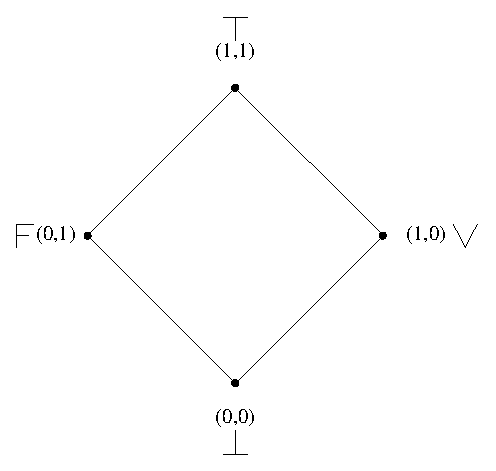
\includegraphics[scale=1.0]{./pic/C421reticuladoHasse.eps}
\label{fig:reticuladoHasse}

{\small Fonte: \cite{JoaoInacio} }
\end{figure}

Para toda proposição $P$ há um par de valores, chamada de anotação, $(\mu , \lambda )$, onde $\mu$ é o grau de evidência favorável e $\lambda $ é o grau de evidência desfavorável, representada como  $P_{( \mu , \lambda )}$ .

%$P_{( \mu , \lambda )}$
Como exemplificação, para uma proposição $P \equiv$ \emph{"A velocidade de rotação do motor atingiu o valor desejado."}, assume-se dois especialistas para realizarem a leitura dos valores da anotação. Em um sistema físico, os especialistas geralmente são sensores, como neste caso, poderia ser um encoder ou sensor óptico como contador de voltas associado a uma base de tempo.

\begin{itemize}
\item 
$\mu$ = grau de evidência favorável (especialista 1), ou seja, com quanto de certeza, em um intervalo fechado $[0,1]$, sendo 0 para grau nulo de certeza e 1 grau máximo de certeza para a dada proposição $P$;

\item
$\lambda$ = grau de evidência desfavorável (especialista 2), ou seja, com quanto de certeza, em um intervalo fechado $[0,1]$, sendo 0 o grau nulo de certeza à evidência desfavorável e 1 o grau máximo de certeza à evidência desfavorável para a dada proposição $P$.

\end{itemize}


Assim, podemos interpretar da seguinte forma os valores da anotação para as posições extremas do reticulado finito de Hasse:

\begin{itemize}
\item 
$(\mu, \lambda ) = (1,0)$ : Há um grau de evidência favorável total e um grau de evidencia desfavorável nulo, ou seja, a afirmação da proposição é máxima e sua negação é nula, assim,  $P$ é \emph{Verdadeira} e \emph{A velocidade de rotação do motor atingiu o valor desejado};

\item 
$(\mu, \lambda ) = (0,1)$ : Há um grau de evidência favorável nulo e um grau de evidencia desfavorável máximo, ou seja, a afirmação da proposição é nula e sua negação é máxima, assim,  $P$ é \emph{Falsa} e \emph{A velocidade de rotação do motor não atingiu o valor desejado};

\item 
$(\mu, \lambda ) = (1,1)$ : Há um grau de evidência favorável máximo e também um grau de evidencia desfavorável máximo, ou seja, a afirmação da proposição é máxima e sua negação também é máxima, assim,  $P$ é \emph{Inconsistente} e \emph{A velocidade de rotação do motor atingiu e não atigiu o valor desejado}, contradição;

\item 
$(\mu, \lambda ) = (0,0)$ : Há um grau de evidência favorável nulo e também um grau de evidencia desfavorável nulo, ou seja, a afirmação da proposição é nula e sua negação também é nula, assim,  $P$ é \emph{Indeterminada} e \emph{A velocidade de rotação do motor nem atingiu o valor desejado e nem não atingiu o valor desejado}, situação paracompleta.

\end{itemize}

Os graus de evidência podem assumir valores não extremos:

\begin{itemize}
\item 
$(\mu, \lambda ) = (0.8,0.3)$ : Crê-se com grau de evidência favorável de 80\% e um grau de evidencia desfavorável de 30\%  que \emph{A velocidade rotação do motor atingiu do valor desejado}.
\end{itemize}

Existe um operador de negação ($\sim $) sobre $\tau$ de forma que :
\begin{center}
\begin{equation}
\sim  : \mid \tau \mid \rightarrow \mid \tau , \sim(\mu, \lambda ) = (\lambda, \mu )
\end{equation}
\end{center}

Então,
\begin{center}
\begin{equation}
P_{(0.8,0.3)} \leftrightarrow \textrm{"   "} \sim P_{(0.3,0.8)}
\end{equation}
\end{center}

\begin{itemize}
\item 
$(\mu, \lambda ) = (0.8,0.3) = \sim (0.3,0.8)$ : Não crê-se que há um grau de evidência favorável de 30\% e um grau de evidencia desfavorável de 80\% que \emph{A velocidade de rotação do motor atingiu do valor desejado}.
\end{itemize}



%%%%%%%%%%%%%%%%%%%%%%%%%%%%%%%%%%%%%%%%%%%%%%%%%%%%%%%%%%%%
\subsection{Quadrado Unitário no Plano Cartesiano - QUPC}
%%%%%%%%%%%%%%%%%%%%%%%%%%%%%%%%%%%%%%%%%%%%%%%%%%%%%%%%%%%%

Uma outra forma de representação da anotação é utilizando o Quadrado Unitário no Plano Cartesiano (QUPC) no qual são transpostos os pontos extremos às respectivas posições de acordo com o par ordenado,  $(\mu, \lambda ) \leftrightarrow (x,y) $, assim o eixo $x$ corresponde ao grau de evidência favorável e o eixo $y$ corresponde ao grau de evidência desfavorável, conforme mostrado na Figura \ref{fig:reticuladoQUPC}.



\begin{figure}[!htb]
\caption{Representação do reticulado no quadrado unitário no plano cartesiano}
\center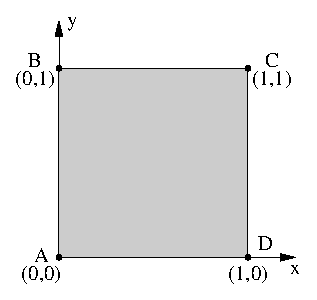
\includegraphics[scale=1.0]{./pic/C422qupc.eps}
\label{fig:reticuladoQUPC}

{\small Fonte: \cite{JoaoInacio} }
\end{figure}

Os pontos extremos assim representam:

\begin{itemize}
\item $A: (0,0) = \bot \Rightarrow $ Paracompleto;
\item $B: (0,1) = F \Rightarrow $ Falso;
\item $C: (1,1) = \top \Rightarrow $ Contradição;
\item $D: (1,0) = V \Rightarrow $ Verdade.
\end{itemize}

O segmento de reta $\overline{BD}$, entre os pontos referentes às condições $Verdade$ e $Falso$, conforme mostrado na Figura \ref{fig:retaPerfeitamenteDefinida}, é denominada de \emph{Reta Perfeitamente Definida} e dada uma anotação $(\mu, \lambda )$ situada nela, a soma das evidências anotadas é sempre o valor unitário do quadro. 

\begin{figure}[!htb]
\caption{Representação da Reta Perfeitamente Definida}
\center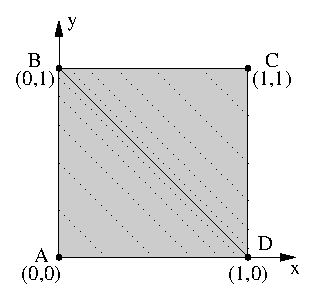
\includegraphics[scale=1.25]{./pic/C424retaPerfeitamenteDefinida.eps}
\label{fig:retaPerfeitamenteDefinida}

{\small Fonte: \cite{JoaoInacio}}
\end{figure}

A relação dos graus de evidência da anotação quando coincidente à Reta Perfeitamente Definida é: 

\begin{center}
\begin{equation}
\mu + \lambda = 1
\label{eq:evidenciaUnitaria1}
\end{equation}
\end{center}

Assim, temos que:

\begin{center}
\begin{equation}
\mu + \lambda - 1 = 0
\label{eq:evidenciaUnitaria}
\end{equation}
\end{center}


Os graus de evidência não precisam apresentar valores complementares, possuem independência entre si, assim das Equações  
\ref{eq:evidenciaUnitaria1} e 
\ref{eq:evidenciaUnitaria} 
é elaborado o conceito de 
\emph{Grau de Contradição}($G_{ct}$), 
e temos que: 

\begin{center}
\begin{equation}
G _{ct} = \mu + \lambda - 1
\label{eq:grauIncerteza}
\end{equation}
\end{center}

pois quanto mais próximo da Reta Perfeitamente Definida, menor é o grau de contradição apresentado pelos graus de evidência, sendo zero quando não houver contradição e o ponto de anotação situar-se sobre a Reta Perfeitamente Definida. 
Quanto mais afastado da Reta Perfeitamente Definida estiver o ponto de anotação, e mais próximo aos pontos A ou C, maior é o Grau de Contradição. 

Quando a anotação estiver situada na região entre os pontos BCD, acima da reta perfeitamente definida, o Grau de Contradição é denominado 
\emph{Grau de Inconsistência} ($G_{it}$), 
e isso ocorre quando, $\mu \ge \lambda $, de forma oposta, quando $\mu < \lambda $ a anotação está situada na região entre os pontos BAD, abaixo da reta perfeitamente definida, e o grau de contradição é denominado 
\emph{Grau de Indefinição} ($G_{id}$), 
então pode-se dizer que:

\begin{center}
\begin{equation}
-1 \le G _{id}  <  0 \le G _{it} \le 1
\label{eq:grauInconsistenciaIndefinicao}
\end{equation}
\end{center}
e
\begin{center}
\begin{equation}
-1 \le G _{ct} \le 1
\label{eq:grauInconsistenciaIndefinicao1}
\end{equation}
\end{center}


O segmento de reta $\overline{ AC }$ , entre os pontos referentes às condições \emph{Paracompleto} e \emph{Contradição}, conforme mostrado na Figura \ref{fig:retaPerfeitamenteIndefinida}, é denominada de \emph{Reta Perfeitamente Indefinida} e dada uma anotação $(\mu, \lambda )$ situada nela, a subtração das evidências anotadas é sempre zero, $\mu = \lambda$, e de forma contrária, quando a anotação está posicionada de forma não coincidente à Reta Perfeitamente Indeterminada, significa que $\mu \neq \lambda$.

\begin{figure}[!htb]
\caption{Representação da Reta Perfeitamente Indefinida}
\center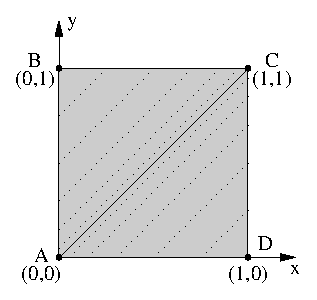
\includegraphics[scale=1.25]{./pic/C426retaPerfeitamenteIndefinida.eps}
\label{fig:retaPerfeitamenteIndefinida}

{\small Fonte: \cite{JoaoInacio} }
\end{figure}

A relação dos graus de evidência para uma anotação cuja posição coincide com a Reta Perfeitamente Indefinida é: 

\begin{center}
\begin{equation}
\mu - \lambda = 0
\label{eq:evidenciaIndefinida}
\end{equation}
\end{center}

De forma análoga ao Grau de Contradição, da Equação \ref{eq:evidenciaIndefinida} é elaborado o conceito de \emph{Grau de Certeza} ($G _c$), assim temos que: 

\begin{center}
\begin{equation}
G _{c} = \mu - \lambda
\label{eq:grauCerteza}
\end{equation}
\end{center}

Quando os graus de evidência, favorável e desfavorável, são iguais, não há certeza em relação à proposição, mas quando são diferentes, alguma certeza pode ser inferida, até a condição máxima onde uma das evidências é total (1) e a outra é nula (0), caracterizando a condição verdadeira ou falsa, afastando o ponto anotado da Reta Perfeitamente Indefinida. 

Quando a anotação situa-se entre os pontos ABC do QUPC, o grau de certeza é denominado \emph{Grau de Falsidade ($G _f$)}, e tal condição ocorre quando $\mu < \lambda $, caso contrário, se $\mu \ge \lambda $, a anotação situa-se entre os pontos ACD do QUPC, e o grau de certeza é denominado \emph{Grau de Verdade ($G _v)$}, então pode-se dizer que:
\begin{center}
\begin{equation}
-1 \le G _{f}  <  0 \le G _{v} \le 1
\label{eq:grauVerdadeFalsidade}
\end{equation}
\end{center}
e
\begin{center}
\begin{equation}
-1 \le G _{c} \le 1
\label{eq:grauCertezaIntervalo}
\end{equation}
\end{center}

Graficamente são representadas como mostra a Figura \ref{fig:retasgcgct}:

\begin{figure}[!htb]
\caption{Representação dos Graus de Certeza e Contradição em um plano cartesiano}
\center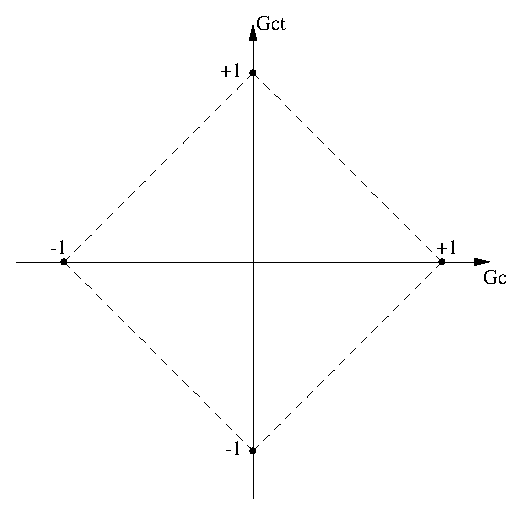
\includegraphics[scale=1.0]{./pic/C428retasgcgct.eps}
\label{fig:retasgcgct}

{\small Fonte: \cite{JoaoInacio}}
\end{figure}

A representação ainda é dividia em algumas partes, dependendo da aplicação, estabelecendo quais são os limites que definem cada estado, Verdadeiro, Falso, Paracompleto, Contradição e outros mais que forem pertinentes à aplicação, estão representados pelas linhas tracejadas na Figura \ref{fig:valorControle} e são definidos como:

\begin{itemize}
\item \emph{V $_{scc}$ : Valor limite superior de Controle de Certeza};
\item \emph{V $_{icc}$ : Valor limite inferior de Controle de Certeza};
\item \emph{V $_{sci}$ : Valor limite superior de Controle de Incerteza};
\item \emph{V $_{sci}$ : Valor limite inferior de Controle de Incerteza}.

\end{itemize}

\begin{figure}[!htb]
\caption{Representação dos valores de controle}
\center\includegraphics[scale=1.0]{./pic/C429valorControle.eps}
\label{fig:valorControle}

{\small Fonte: \cite{JoaoInacio}}
\end{figure}

Uma divisão em 12 partes é mostrada na Figura \ref{fig:reticuladoLPA2v} com seus respectivos estados intermediários definidos conforme \citeauthor{JoaoInacio}(\citeyear{JoaoInacio}), sendo 4 regiões extremas:


%\begin{figure}[!htb]
%\center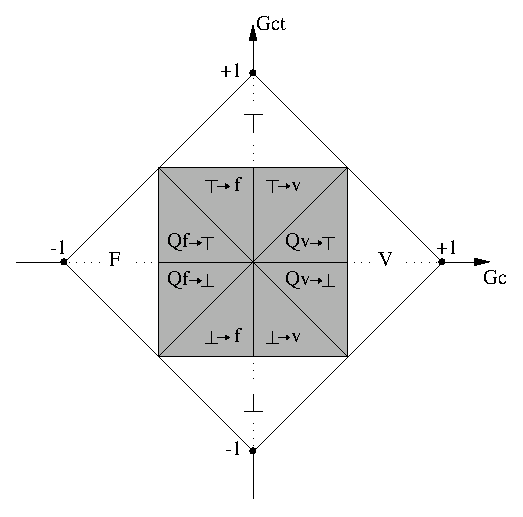
\includegraphics[scale=1.5]{./pic/C430gcgct.eps}
%\caption{Representação do reticulado da LPA2v subdividido em 12 regiões}
%\label{fig:reticuladoLPA2v}
%\end{figure}


\begin{figure}[!h]
\centering
\caption{Representação do reticulado da LPA2v subdividido em 12 regiões}
\begin{tikzpicture}[scale=1.0]
\tikzset{ >=latex, inner sep=0pt, outer sep=0pt,  }

%\draw [lightgray, dashed](0,0) grid (10,10);

\node [fill=black, circle] (V) at (9,5) {:};
\node [fill=black, circle] (F) at (1,5) {:};
\node [fill=black, circle] (T) at (5,9) {:};
\node [fill=black, circle] (L) at (5,1) {:};

\node [fill=black, circle] (N) at (5,7) { };
\node [fill=black, circle] (S) at (5,3) { };
\node [fill=black, circle] (E) at (7,5) { };
\node [fill=black, circle] (W) at (3,5) { };

\node [fill=black, circle] (NE) at (7,7) { };
\node [fill=black, circle] (SE) at (7,3) { };
\node [fill=black, circle] (NW) at (3,7) { };
\node [fill=black, circle] (SW) at (3,3) { };


%\draw [dashed] (F) -- (V);
%\draw [dashed] (T) -- (L);
\draw [->, thick] (V)   -- (10,5);
\draw [    thick] (0,5) -- (F);
\draw [->, thick] (T)   -- (5,10);
\draw [    thick] (5,0) -- (L);

\draw [thick] (V) -- (T);
\draw [thick] (T) -- (F);
\draw [thick] (F) -- (L);
\draw [thick] (L) -- (V);

\draw [thick] (N) -- (S);
\draw [thick] (E) -- (W);
\draw [thick] (NE) -- (SW);
\draw [thick] (SE) -- (NW);


\draw[thick] (SW) rectangle (NE);
\fill[nearly transparent] (SW) rectangle (NE);

\node at (8,5) {V};
\node at (2,5) {F};
\node at (5,8) {$\top$};
\node at (5,2) {$\bot$};

\node at (6.2,5.3) {Qv$\rightarrow\top$ };
\node at (6.2,4.7) {Qv $\rightarrow  \bot$ };
\node at (3.8,5.3) {Qf $\rightarrow  \top$ };
\node at (3.8,4.7) {Qf $\rightarrow  \bot$ };
\node at (4.2,6.6) {$\top \rightarrow $ f };
\node at (5.8,6.6) {$\top \rightarrow $ v };
\node at (4.2,3.4) {$\bot \rightarrow $ f };
\node at (5.8,3.4) {$\bot \rightarrow $ v };

\node at (10,4.5) {$G_{c}$};
\node at (5.5,10) {$G_{ct}$};

\node at (4.5,9.2) {$+1$};
\node at (9.0,5.5) {$+1$};
\node at (5.5,1.0) {$-1$};
\node at (1.0,4.5) {$-1$};

\end{tikzpicture}
\label{fig:reticuladoLPA2v}

{\small Fonte: \cite{JoaoInacio} }
\end{figure}




\begin{itemize}
\item V : Verdadeiro;
\item F : Falso;
\item $\top$ : Contradição;
\item $\bot$ : Paracompleto.
\end{itemize}
e 8 regiões intermediárias: 
\begin{itemize}
\item Qv $\rightarrow  \top$ : Quase Verdade tendendo à Contradição;
\item Qv $\rightarrow  \bot$ : Quase Verdade tendendo à  Paracompleto;
\item Qf $\rightarrow  \top$ : Quase Falso tendendo à Contradição;
\item Qf $\rightarrow  \bot$ : Quase Falso tendendo à Paracompleto;
\item $\top \rightarrow $ f : Contradição tendendo à Falso;
\item $\top \rightarrow $ v : Contradição tendendo à Verdadeiro;
\item $\bot \rightarrow $ f : Paracompleto tendendo à Falso;
\item $\bot \rightarrow $ v : Paracompleto tendendo à Verdadeiro.

\end{itemize}

O reticulado subdividido em 12 regiões como mostrado, é aplicado em situações nas quais a tomada de decisão utiliza estados discretos bem definidos para atuação, onde para cada posição da anotação e respectivamente um estado do reticulado, uma ação é tomada, assim sendo, a quantidade de subdivisões está fortemente dependente da aplicação.


O reticulado pode ser dividido de outras formas, dependendo dos limites dos Graus de Certeza e Contradição que o sistema permite. A Figura \ref{fig:reticuladoLPA2v2} mostra uma das possibilidades com a representação de 8 regiões do reticulado. 


\begin{figure}[!h]
\centering
\caption{Representação do reticulado da LPA2v subdividido em 8 regiões}
\begin{tikzpicture}[scale=1.0]
\tikzset{ >=latex, inner sep=0pt, outer sep=0pt,  }

%\draw [lightgray, dashed](0,0) grid (10,10);

\node at (10,4.5) {$G_{c}$};
\node at (5.5,10) {$G_{ct}$};

\node at (4.5,9.2) {$+1$};
\node at (9.0,5.5) {$+1$};
\node at (5.5,1.0) {$-1$};
\node at (1.0,4.5) {$-1$};

\node [fill=black, circle] (V) at (9,5) {:};
\node [fill=black, circle] (F) at (1,5) {:};
\node [fill=black, circle] (T) at (5,9) {:};
\node [fill=black, circle] (L) at (5,1) {:};

\node [fill=black, circle] (N) at (5,7) { };
\node [fill=black, circle] (S) at (5,3) { };
\node [fill=black, circle] (E) at (7,5) { };
\node [fill=black, circle] (W) at (3,5) { };

\node [fill=black, circle] (NE) at (8,6) { };
\node [fill=black, circle] (SE) at (8,4) { };
\node [fill=black, circle] (NW) at (2,6) { };
\node [fill=black, circle] (SW) at (2,4) { };

\draw [->, thick] (V)   -- (10,5);
\draw [    thick] (0,5) -- (F);
\draw [->, thick] (T)   -- (5,10);
\draw [    thick] (5,0) -- (L);

\draw [thick] (V) -- (T);
\draw [thick] (T) -- (F);
\draw [thick] (F) -- (L);
\draw [thick] (L) -- (V);

\draw [thick] (NE) -- (SW);
\draw [thick] (SE) -- (NW);

\draw[thick] (SW) rectangle (NE);
\fill[nearly transparent] (SW) rectangle (NE);

\node at (8.5,5.0) {V};
\node at (1.5,5.0) {F};
\node at (5.0,8.0) {$\top$};
\node at (5.0,2.0) {$\bot$};

\node at (7.0,5.0) {Qv};
\node at (3.0,5.0) {Qf};
\node at (5.0,5.5) {Q$\top$};
\node at (5.0,4.5) {Q$\bot$};

\end{tikzpicture}
\label{fig:reticuladoLPA2v2}

{\small Fonte: Próprio autor}
\end{figure}

Sendo 4 regiões extremas,
\begin{itemize}
\item V : Verdadeiro;
\item F : Falso;
\item $\top$ : Contradição;
\item $\bot$ : Paracompleto.
\end{itemize}
e 4 regiões intermediárias: 
\begin{itemize}
\item Qv: Quase Verdade;
\item Qf: Quase Falso;
\item Q$\top$: Quase Contradição;
\item Q$\bot$: Quase Paracompleto.

\end{itemize}


%###

É possível e desejável que se possa utilizar um valor resultante que exclua os efeitos das incertezas ou contradições, 
como é citado por 
\citeauthor{JairJoaoGermano}(\citeyear{JairJoaoGermano}): 
\begin{citacao}
{
"Um sistema de decisão capaz de analisar dados originários de Conhecimento Incerto terá maior robustez quando, 
ao final da análise,
apresentar um resultado que represente o valor de certeza puro, 
isto é, não contaminado pelos efeitos das incertezas."
}
\end{citacao}

O valor que elimina o efeito da incerteza é denominado \emph{Grau de Certeza Real - G$_{CR}$} 
e é calculado pela distância (D) do Ponto de análise, $(G_c,G_{ct})$, 
em relação ao ponto de máximo Grau de Certeza $V$, 
no vértice direito do reticulado, 
conforme mostrado na Figura \ref{fig:reticuladoGer}.


\begin{figure}[!h]
\centering
\caption{Representação do Grau de Certeza Real no reticulado }
\begin{tikzpicture}[scale=1.0]
\tikzset{ >=latex, inner sep=0pt, outer sep=0pt,  }

%\draw [lightgray, dashed](0,0) grid (10,10);

\node at (10,4.5) {$G_{c}$};
\node at (5.5,10) {$G_{ct}$};

\node at (4.5,9.2) {$+1$};
\node at (9.0,5.5) {$+1$};
\node at (5.5,1.0) {$-1$};
\node at (1.0,4.5) {$-1$};

\node at (9.0,4.5) {V};
\node at (1.0,5.5) {F};
\node at (5.5,9.0) {$\top$};
\node at (4.5,1.0) {$\bot$};

\node [fill=black, circle] (V) at (9,5) {:};
\node [fill=black, circle] (F) at (1,5) {:};
\node [fill=black, circle] (T) at (5,9) {:};
\node [fill=black, circle] (L) at (5,1) {:};

\draw [thick] (V) -- (T);
\draw [thick] (T) -- (F);
\draw [thick] (F) -- (L);
\draw [thick] (L) -- (V);

\draw [->, thick] (V)   -- (10,5);
\draw [    thick] (0,5) -- (F);
\draw [->, thick] (T)   -- (5,10);
\draw [    thick] (5,0) -- (L);

\draw [lightgray,dashed] (V) -- (F);
\draw [lightgray,dashed] (T) -- (L);

\node [fill=black, circle] (P) at (6.0,7.0) {:};
\node [fill=gray,  circle] (p) at (5.4,5.0) [gray] {:};
\node [fill=black, circle] (r) at (6.0,5.0) [gray]{.};

\draw [blue,ultra thick] (P) -- (V);
\draw [green ] (r) -- (V);
\draw [yellow] (P) -- (r);
%\draw [green,ultra thick] (9.0,4.9) -- (5.4,4.9);

\draw [red, ultra thick,<-]  (p) to [out=85, in=236] (P);

\node at (7.0,6.0) [blue]{D};
\node at (5.7,7.4) {($G_c$,$G_{ct}$)};
\node at (5.5,4.6) {$G_{CR}$};

\end{tikzpicture}
\label{fig:reticuladoGer}

{\small Fonte: \cite{JairJoaoGermano}}
\end{figure}


O Grau de Certeza Real ($G_{CR}$) 
é calculado utilizando o Teorema de Pitágoras para achar a distância D 
conforme Equação \ref{eq:grauCertezaReal}. 

\begin{center}
\begin{equation}
D = \sqrt{(1-|G_c|)^2+G_{ct}^2}
\label{eq:grauCertezaReal}
\end{equation}
\end{center}

Para valores de $G_c \geq 0$: 

\begin{center}
\begin{equation}
G_{CR} = (1-D)
\end{equation}
\end{center}

Para valores de $G_c < 0$:

\begin{center}
\begin{equation}
G_{CR} = (D-1)
\end{equation}
\end{center}


Tanto o Grau de Evidência Real quanto os estados ou regiões do reticulado 
podem ser utilizados para realizar o controle dos mais diversos tipos de sistemas, 
dependendo apenas do tipo de controle e de sistema que deve ser implementado. 

%%%%%%%%%%%%%%%%%%%%%%%%%%%%%%%%%%%%%%%%%%%%%%%%%%%%%%%%%%%%
\subsection{A LPA2v aplicada em Controle}
%%%%%%%%%%%%%%%%%%%%%%%%%%%%%%%%%%%%%%%%%%%%%%%%%%%%%%%%%%%%

Os Sistemas Inteligentes estão cada vez mais presentes 
em diversas aplicações modernas, 
e segundo \citeauthor{JISF2011}(\citeyear{JISF2011}), 
há um predomínio de Lógicas Não-Clássicas no suporte à tomada de decisão desses sistemas. 
O sucesso na aplicação de técnicas como a LPA2v, 
que é uma extensão da Lógica Paraconsistente Anotada, 
se dá em grande medida pelo uso de 
algorítmos baseados em estudos dos reticulados representativos e 
efetiva tradução matemática 
gerando um modelo eficiente aplicado em situações reais.

Assumindo que a lógica filosófica trata da descrição formal da linguagem natural 
e define a sua estrutura de declaração, então, 
sendo encontrada a linguagem adequada 
é possível traduzir o raciocínio formal em LPA, 
modelando raciocínios com a possibilidade de 
tratar contradições ou incoerências, 
e trabalhar com situações reais, 
da mesma forma que o Modelo Clássico, 
que aplica regras computacionais, 
a LPA2v possui um conjunto de axiomas e regras de inferência 
que possibilitam um raciocínio válido em situações reais.

\subsubsection{Robótica}

Os algorítmos baseados no estudo do Reticulado Representativo gera 
Estados Lógicos Paraconsistentes através da 
descrição do algorítmo Para-Analisador da LPA2v, 
possibilitando que o sistema receba informação 
através dos graus de evidência ($\mu, \lambda$), 
processe os graus de certeza e contradição ($G_c$ e $G_{ct}$) e 
chegue a uma conclusão, de alta contradição e busque por mais dados ou 
um alto grau de certeza, que de um modo geral, implica em tomar uma ação. 

Os Graus de Certeza e Contradição podem gerar um Grau de Certeza Real, 
que pode servir de entrada para outra célula ou 
Nó de Análise Paraconsistente (NAP), 
possibilitando uma rede de análises para a tomada de decisão,
como apresentado pelo Professor Dr. João Inácio da Silva Filho 
com a construção do Robô Emmy, 
desenvolvendo e aplicando tais técnicas aplicadas ao sistema de movimentação.

\subsubsection{Engenharia de Produção}

A LPA2v pode ser aplicada em diversas áreas 
sendo um outro exemplo a sua aplicação na 
área de Eng. de Produção, 
como é mostrado no artigo de 
\citeauthor{FabioIsraelJair}(\citeyear{FabioIsraelJair}), 
que mostram um estudo para avaliação do projeto de uma fábrica, 
como são selecionadas as variáveis relevantes, ou fatores, como são chamados,
níveis de exigência para tomada de decisão, 
atribuição de pesos aos fatores de decisão, 
para obtenção dos graus de crença e descrença. 
Construção de uma base de dados, sua pesquisa e obtenção dos resultados.
Análise dos resultados e fidedignidade utilizando um 
Método de Análise pelo Baricentro.

\subsubsection{Logística}

No segmento logístico pode-se citar a dissertação do 
Profº Me. Vander Célio Nunes (\cite{Vander}), 
que aplicou a LPA2v ao processo de paletização 
através da medição de peças e do tratamento de incertezas 
relacionadas a possibilidade de seu depósito ou encaixe na pilha de palets, 
levando à otimização de cargas armazenadas em um determinado espaço. 
O seu trabalho, utilizando uma célula de manufatura 
com um braço robótico industrial, 
permite a extrapolação da sua aplicação para portos e armazens de containers.


\subsubsection{Sistema de Controle Híbrido}

No segmento de controle, a LPA2v é utilizada em conjunto com um 
sistema Proporcional-Integral - PI de modo que 
as ações convencionais são executadas pelo bloco PI, 
mas são estruturadas utilizando a LPA2v no 
tratamento dos sinais externos. 
A implementação é feita por 
\citeauthor{Marcelo}(\citeyear{Marcelo}) 
em uma planta de controle de nível e um
controlador lógico programável. 
O sistema Híbrido é posto em operação e 
comparado com técnicas consagradas como o 
controle puramente PI, ajustado com o
método de Ziegler-Nichols e com o 
método interno do controlador. 




%%%%%%%%%%%%%%%%%%%%%%%%%%%%%%%%%%%%%%%%%%%%%%%%%%%%%%%%%%%%
%%%%%%%%%%%%%%%%%%%%%%%%%%%%%%%%%%%%%%%%%%%%%%%%%%%%%%%%%%%%






\chapter[Metodologia]{3. Metodologia}
Para o desenvolvimento deste trabalho foram dadas prioridade e preferência para a utilização de um sistema embarcado de núcleo ARM, com o intúito de desenvolver as capacidades de operar tal tecnologia de processamento, trabalhando com sistema eletrônico simples de fácil acesso mas que atende às necessidades do projeto, bem como a utilização de ferramentas de uso livre.









\section{Materiais}

O protótipo físico foi constuído baseado em um microcontrolador da família Texas Instruments, modelo $Tiva^{TM}$ TM4C123GH6PM, drive para acionamento do tipo \emph{Pulse Width Modulation}(PWM) do motor com circuito integrado de tecnologia CMOS (IRF540), motor de corrente contínua acoplado a um CD, com uma etiqueta, Figura \ref{fig:discoSensor}, para acionar o sensor óptico e servir de indicador para contagem de giros do motor. Fonte de alimentação chaveada de 12V 10W. A maior parte do sistema pode ser visto na Figura \ref{fig:discoSensorGeral} .


\begin{figure}[!htb]
\center
\caption{Visão geral do sistema }
\subfloat[]{
	\label{fig:discoSensor}
	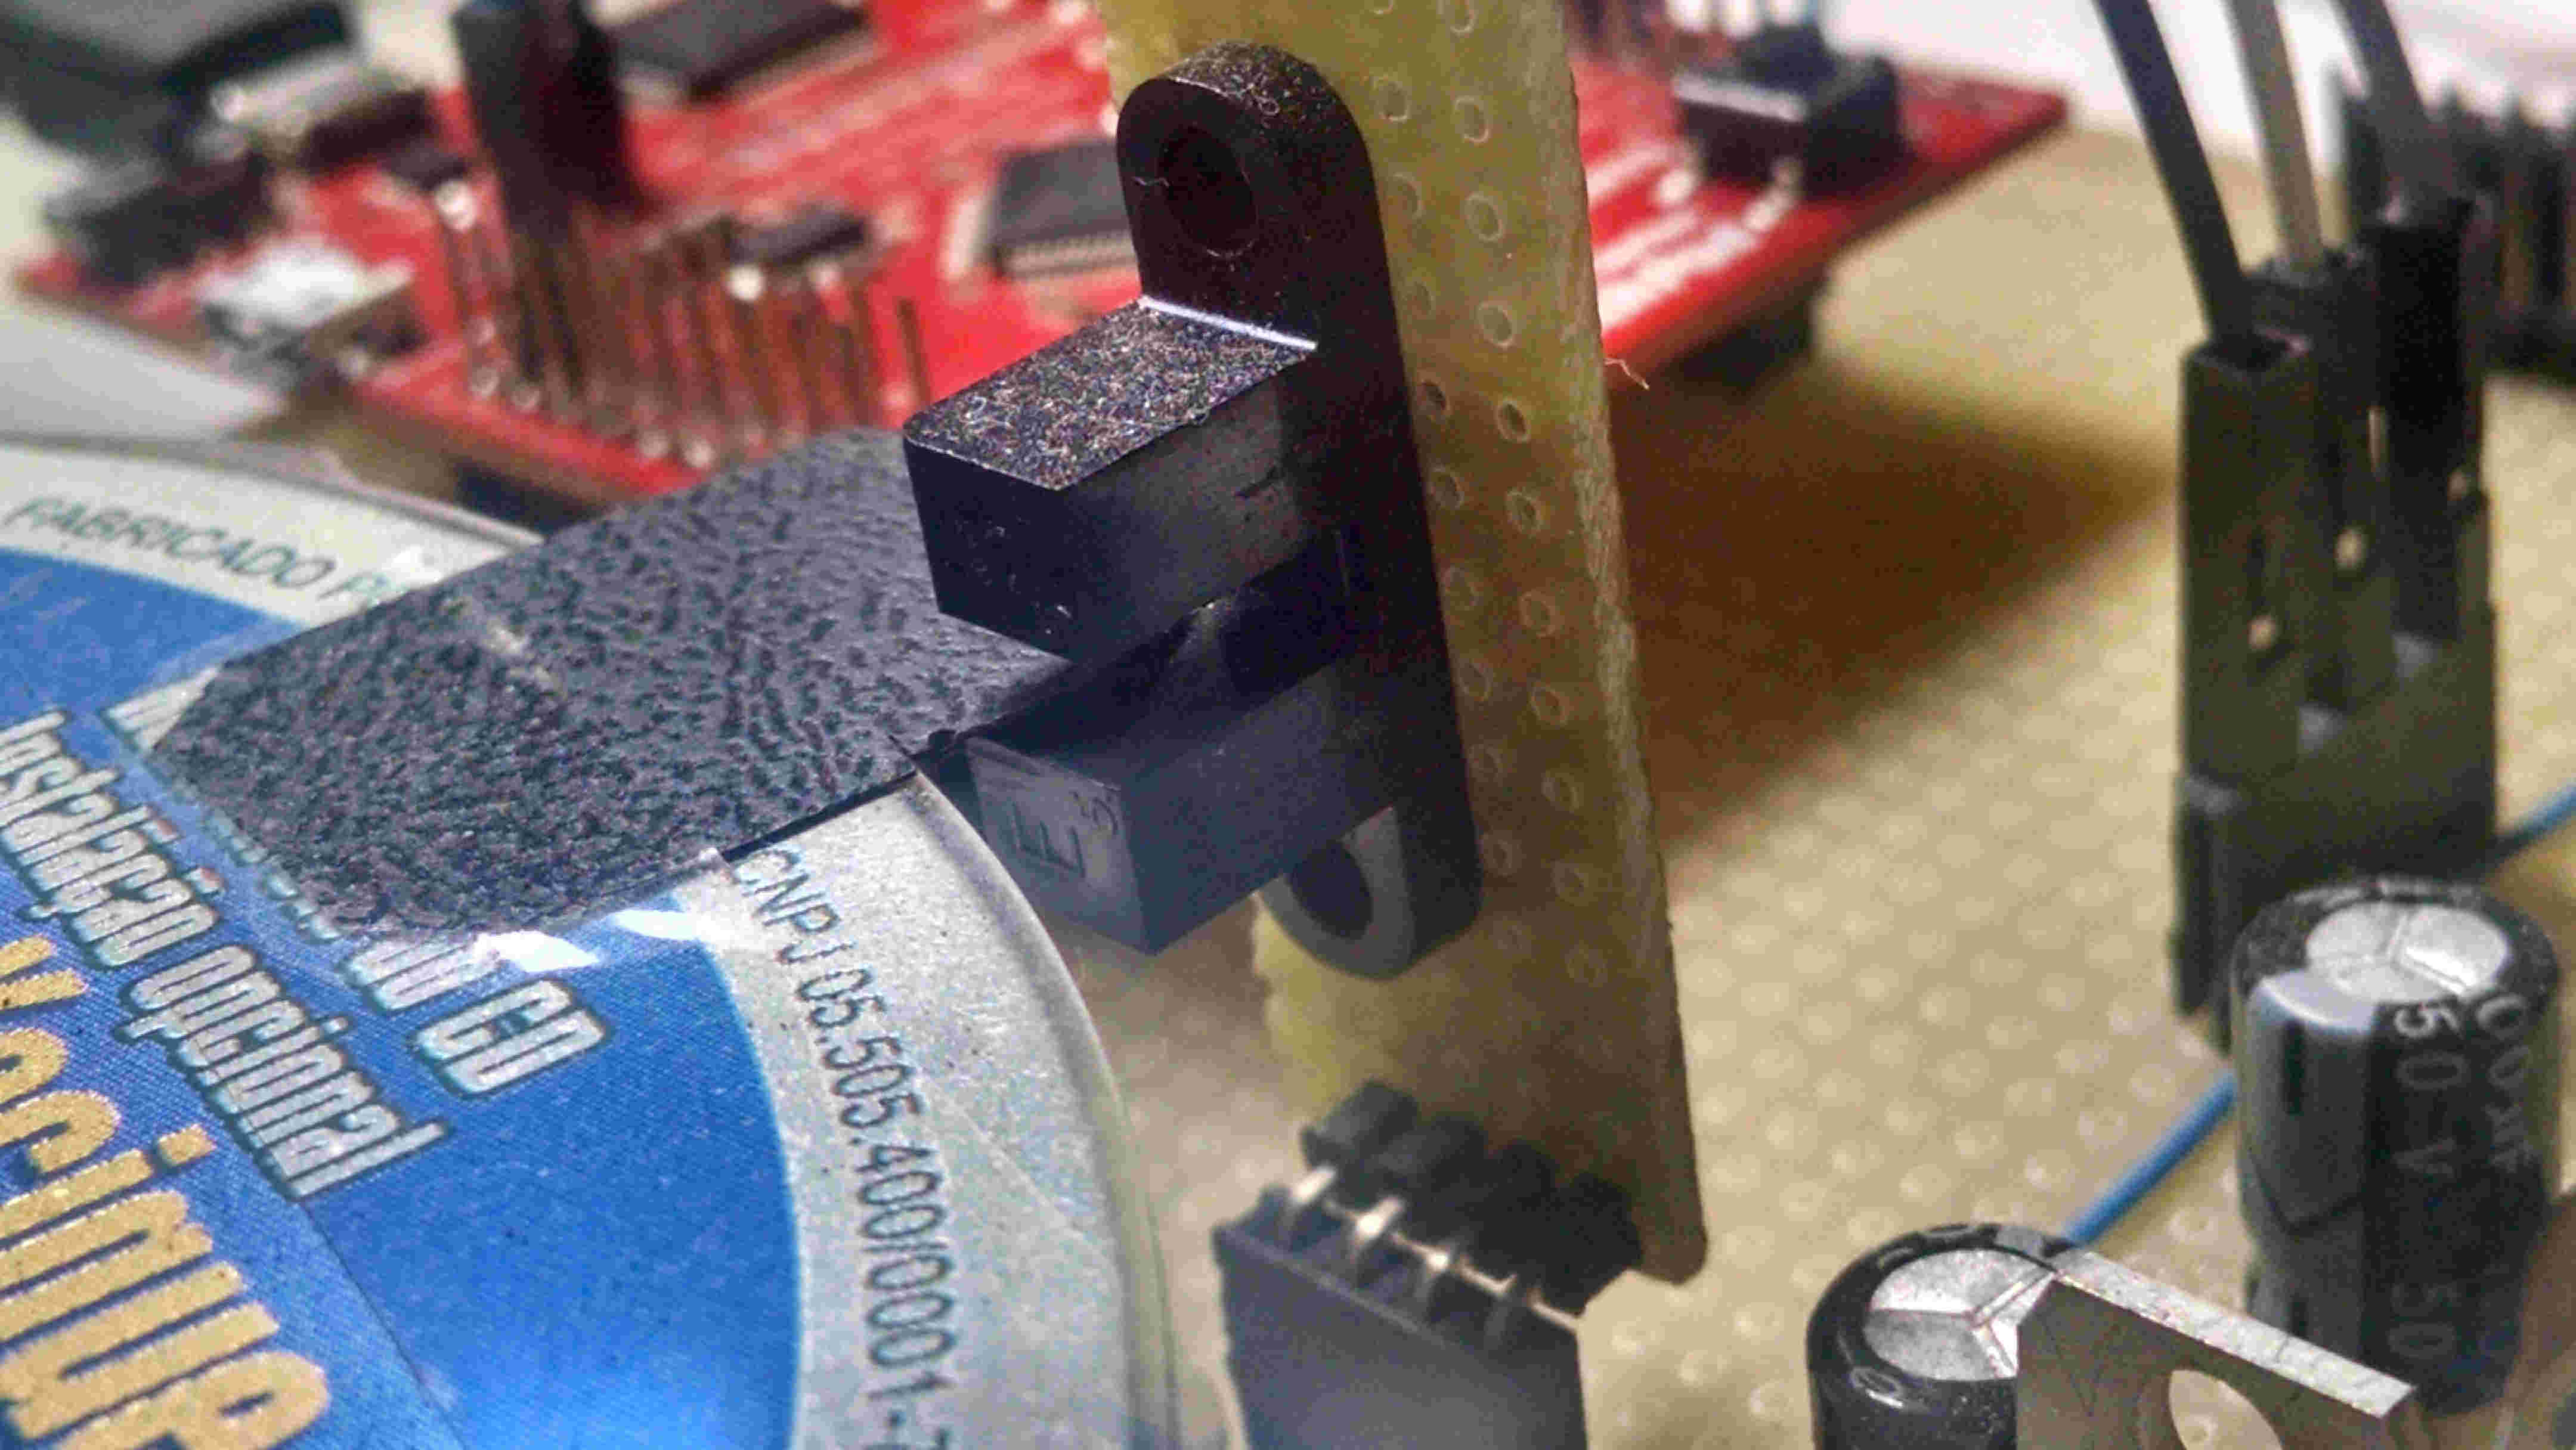
\includegraphics[scale=0.07, angle=0, clip=true, trim=300 200 1200 200]{./imagens/discoSensor.jpg}
	}
\subfloat[]{ 
	\label{fig:discoSensorGeral} 
	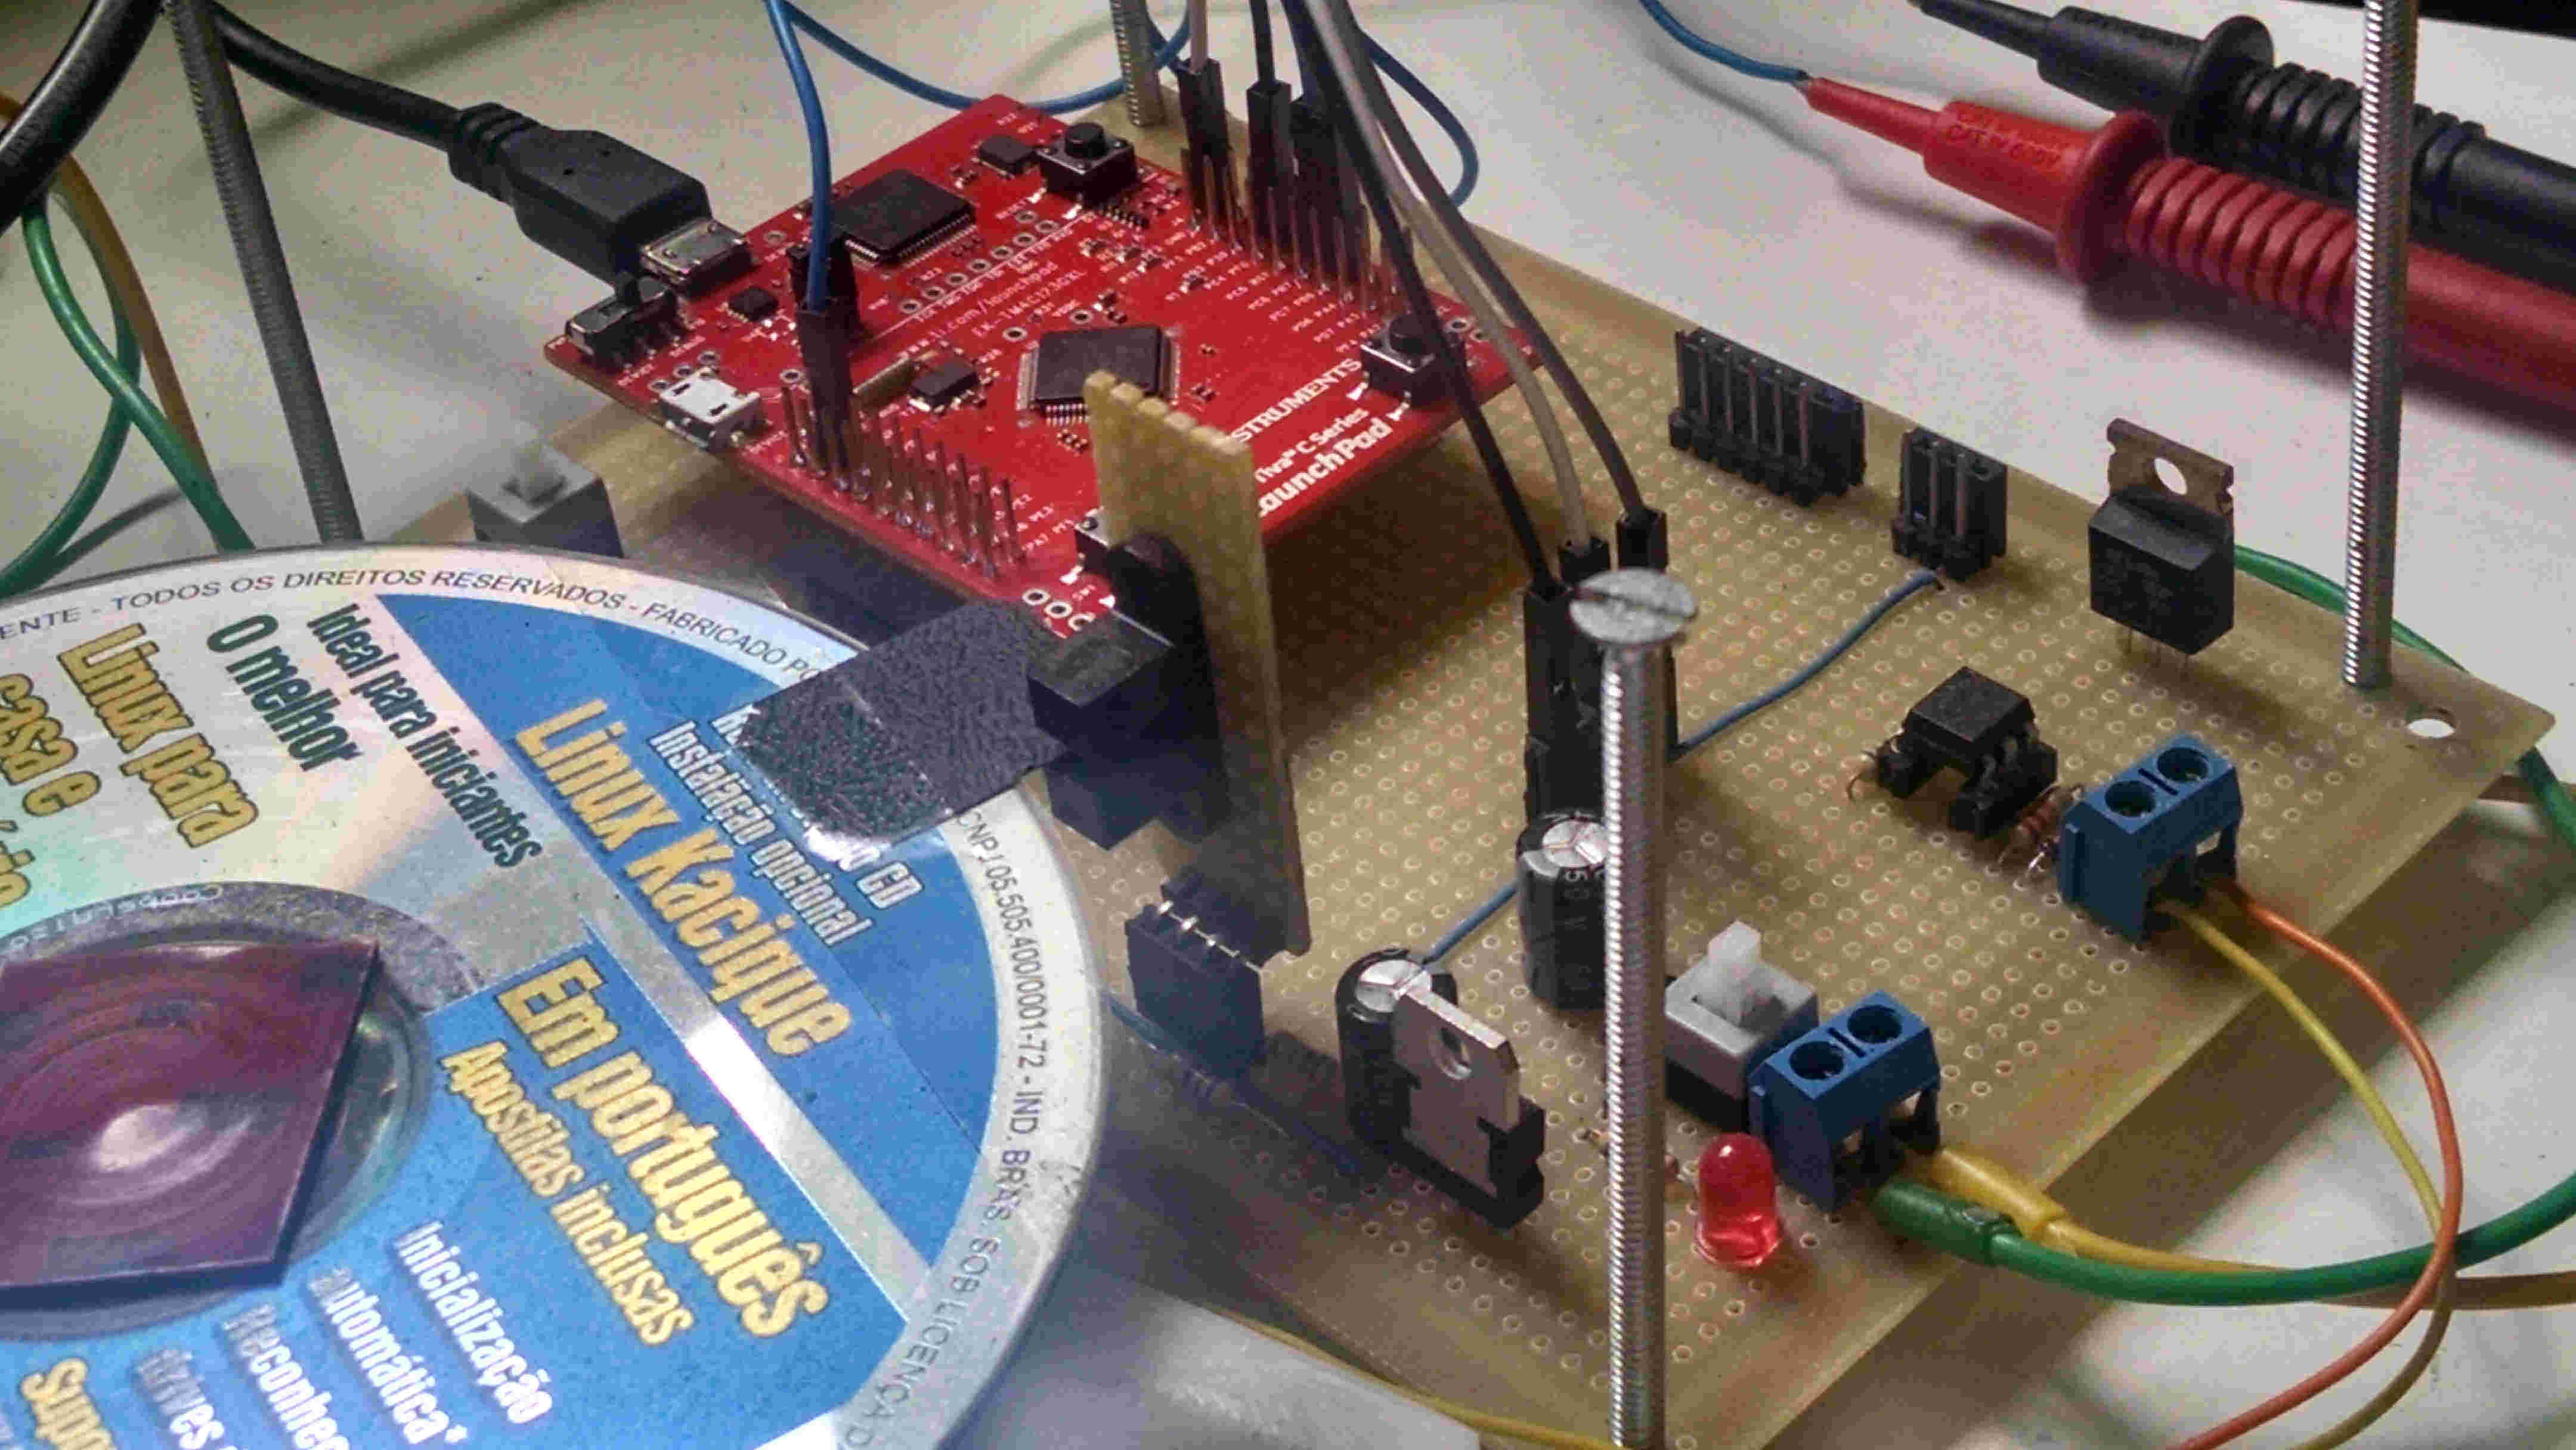
\includegraphics[scale=0.07, angle=0, clip=true, trim=300 200 400 200]{./imagens/discoSensorGeral.jpg} 
	}

{\small Figure: Próprio autor}
\end{figure}

As ferramentas de software utilizadas foram:

\begin{itemize}
\item Sistema Operacional GNU/Linux Debian 8(Jessie);
\item GNOME Shell;
\item Editores de texto e códigos fonte VIM e Emacs;
\item Compilador GCC para ARM (arm-none-eabi-gcc);
\item GNU Make;
\item Processador de texto \LaTeX - pdfTEX; 
\item Pacotes geradores de figuras TikZ, PGF e GNU pic(Groff);
\item Gerador de gráficos GNUPlot;
\item Teminal de comunicação Minicom;
\item Gravador para microcontrolador ARM LM4Flash.
\end{itemize}





\section{ Métodos }

Os métodos utilizados para a validação do objetivo do projeto devem aferir quão próximo o resultado obtido empiricamente foi do objetivo esperado, de modo que as expectativas referentes aos objetivos propostos sejam atendidos ou sua negação seja devidamente exclarecidas. 

Basicamente foram realizados os seguintes passos:

\begin{itemize}
\item Levantamento de um modelo matemático do sistema protótipo utilizado;
\item Aferição da qualidade desse modelo, com erro percentual médio menor do que 5\%, considerando um sistema não crítico;
\item Definição dos requisitos de desempenho do sistema;
\item Comparação dos resultados obtidos empiricamente com os requisitos de desempenho do sistema.
\end{itemize}




\subsection{ Obtenção de um modelo do processo }

Para melhor compreensão dos modelos dinâmicos dos sistemas, é utilizado o Diagrama de blocos do comportamento do sistema em malha aberta, conforme Figura \ref{fig:AcaoMalhaAberta}\cite{Ogata}.


\begin{comment}


\begin{figure}[!htb]
\centering
\caption{ Diagrama de blocos de sistema de controle em malha aberta}
\begin{tikzpicture}[scale=0.85]
%\draw [lightgray](0,0) grid (15,2);
\draw (0,1) -- (3,1);
\draw [black, thick](3,0) rectangle (6, 2) ; 
\draw (6,1) -- (9,1);
\draw [black, thick](9,0) rectangle (12, 2) ; 
\draw (12,1) -- (15,1);

\draw [fill]( 3,1) -- ( 2.8, 1.1) -- ( 2.8,0.9) -- ( 3,1);
\draw [fill]( 9,1) -- ( 8.8, 1.1) -- ( 8.8,0.9) -- ( 9,1);
\draw [fill](15,1) -- (14.8, 1.1) -- (14.8,0.9) -- (15,1);

\node at ( 4.5, 1){Controlador};
\node at (10.5, 1){Planta};
\node [above] at ( 1.5,1){Valor de};
\node [below] at ( 1.5,1){Referência};
\node [above] at ( 7.5,1){Variável};
\node [below] at ( 7.5,1){Manipulada};
\node [above] at (13.5,1){Variável};
\node [below] at (13.5,1){Controlada};
\end{tikzpicture}
\label{fig:malhaAberta}

{\small Fonte: \cite{Ogata}}
\end{figure}

\end{comment}

Utilizando variáveis para cada elemento do Diagrama de blocos, de forma a representá-los nas equações, temos então que:



\begin{figure}[!htb]
\centering
\caption{ Sistema de controle em malha aberta}
\begin{tikzpicture}[scale=0.85]
%\draw [lightgray](0,0) grid (15,2);
\draw (0,1) -- (3,1);
\draw [black, thick](3,0) rectangle (6, 2) ; 
\draw (6,1) -- (9,1);
\draw [black, thick](9,0) rectangle (12, 2) ; 
\draw (12,1) -- (15,1);

\draw [fill]( 3,1) -- ( 2.8, 1.1) -- ( 2.8,0.9) -- ( 3,1);
\draw [fill]( 9,1) -- ( 8.8, 1.1) -- ( 8.8,0.9) -- ( 9,1);
\draw [fill](15,1) -- (14.8, 1.1) -- (14.8,0.9) -- (15,1);

\node at ( 4.5, 1.4){Controlador};
\node at ( 4.5, 0.6){f(t)};
\node at (10.5, 1.4){Planta};
\node at (10.5, 0.6){g(t)};
\node [above] at ( 1.5,1){r(t)};
\node [above] at ( 7.5,1){u(t)};
\node [above] at (13.5,1){c(t)};
\end{tikzpicture}
\label{fig:AcaoMalhaAberta}

{\small Fonte: Próprio autor}
\end{figure}


Onde: 

%\begin{itemize}
%\item 
\hspace{1cm} $r(t)$: Valor de Referência em rotações por segundo [rps];

%\item 
$\hspace{1cm} f(t)$: Controlador que converte rps em \% PWM para acionar o motor;

%\item 
$\hspace{1cm} u(t)$: Variável Manipulada é o valor percentual do PWM;

%\item 
$\hspace{1cm} g(t)$: Planta ou Processo formado pelo motor DC com o disco acoplado no eixo;

%\item 
$\hspace{1cm}  c(t)$: Variável Controlada é a velocidade de rotação do eixo em rps.

%\end{itemize}



O sistema físico aqui estudado possui comportamento exponencial que pode ser descrito pela equação \ref{eq:ftSistOrdem1}. 






\begin{equation}
	 \frac{d c(t)}{dt} + c(t) = r(t) \rightarrow  \mathscr{L} \to \frac{C(s)}{R(s)} = \frac{K}{s + a} 
\label{eq:ftSistOrdem1}
\end{equation}

Onde:

\setlength{\parindent}{2cm}

$t$ : tempo,$ r(t) = 0$ , para t $<$ 0;

$\mathscr{L}$ : Operador de Laplace;

$c(t)$ : Variável controlada no domínio do tempo;

$C(s)$ : Variável controlada no domínio da frequência;

$r(t)$ : Valor de referência (\emph{setpoint}) no domínio do tempo;

$R(s)$ : Valor de referência (\emph{setpoint}) no domínio da frequência.

$K$ : Constante de proporcionalidade;

$s$ : Variável complexa de Laplace;

$a$ : Polo da função.
\setlength{\parindent}{1cm}



Sendo assim, para um estímulo de entrada do tipo \textbf{degrau}, com amplitude \textbf{A}, temos $ R(s) = \frac{A}{s}$ e aplicando a Transformada Inversa de Laplace:

\begin{equation}
C(s) = \frac{K}{s+a} \frac{A}{s} \rightarrow \mathscr{L}^{-1} \to c(t) = \frac{K A}{a} (1 - e^{-at})
\label{eq:degrauA}
\end{equation}

A Figura \ref{fig:degrauA} mostra um sinal do tipo degrau com amplitude \textbf{A} aplicado ao sistema de teste, que responde conforme um sistema de primeira ordem como mostrado na Figura \ref{fig:cRegime}. 


%A partir de um determinado instante de tempo, entra em regime constante ($c_{reg}$), alcançando o valor de referência dado pelo degrau de amplitude A. Assim quando $ t \rightarrow \infty $  então $ c_{reg} \rightarrow A $:




\begin{figure}[!htb]
\centering
\caption{Sistema de Primeira Ordem}
\subfloat[Sinal de entrada tipo degrau com amplitude A]{\label{fig:degrauA}
\begin{tikzpicture}[scale=0.75]
\draw [lightgray, dashed](0,0) grid (8.8,5.8);
\draw [->] (0,0) -- (9,0);
\draw [fill] (0,6.2) -- (-0.1, 5.8) -- (0.1,5.8) -- (0,6.2);
\draw [->] (0,0) -- (0,6);
\draw [fill] (9.2,0) -- (8.8,0.1) -- (8.8,-0.1)--(9.2,0.0);
\node at (9.0,-0.5) {$t$};
\node at (0.2,6.5) {$r(t)$};
\draw [red, ultra thick] (0.0,5.0) -- (9.0,5.0);
\draw [red, ultra thick] (0.0,0.0) -- (0.0,5.0);
\node at (-0.5,5.0)[red]{$A$};
\end{tikzpicture} }
\subfloat[Resposta transitória e regime de acomodação]{\label{fig:cRegime}
\begin{tikzpicture}[scale=0.75]
\draw [lightgray, dashed](0,0) grid (8.8,5.8);
\draw [->] (0,0) -- (9,0);
\draw [fill] (0,6.2) -- (-0.1, 5.8) -- (0.1,5.8) -- (0,6.2);
\draw [->] (0,0) -- (0,6);
\draw [fill] (9.2,0) -- (8.8,0.1) -- (8.8,-0.1)--(9.2,0.0);
\node at (9.0,-0.5) {$t$};
\node at (0.2,6.5) {$c(t)$};
\node at (-0.5,5.0)[blue]{$C_{reg}$};
\draw [blue, ultra thick] (0,0) to [out=85, in=180] (6,5);
\draw [blue, ultra thick] (6,5) -- (9,5);
\end{tikzpicture}}
\label{fig:sistPrimeiraOrdem}

{\small Fonte: Próprio autor}
\end{figure}

%\begin{equation}
%c_{reg} = \lim_{t \rightarrow \infty} \frac{KA}{a}(1-e^{-at}) = \frac{KA}{a}
%\label{eq:cregime}
%\end{equation}



%Aplicando o Teorema do Valor Final pode-se ver que o \emph{$c_{reg}$} estabiliza em um valor constante como mostrado pela Equação \ref{eq:teoremaValorFinal}:

%\begin{equation}
%C_{reg} = \lim_{s \rightarrow 0} sC(s) = \lim_{s \rightarrow 0} s\ \frac{K}{s+a}\frac{A}{s} = \frac{KA}{a}
%\label{eq:teoremaValorFinal}
%\end{equation}



Matematicamente, quanto maior o valor de \emph{t} na Equação \ref{eq:degrauA}, o resultado da exponenencial tende a zero, levando a um resultado que depende apenas das constantes para o valor de referência. 

Tomando $t= \frac{1}{a} = a^{-1} = \tau$ para gerar um valor conhecido em $e^{-at}$, da Equação \ref{eq:degrauA} temos:


\begin{equation}
c(a^-1) = \frac{KA}{a}(1-e^{-(a.a^{-1})}) = \frac{KA}{a}(1-e^{-1}) = \frac{KA}{a}.0,63 = 0,63 . C_{reg}
\end{equation}

A Figura \ref{fig:constTempo} mostra a constante de tempo $\tau$, que é atingida quando o sistema alcança 63\% do seu valor de regime. Como sabemos que $\tau = \frac{1}{a}$, então o polo do sistema, que leva o denominador da Equação \ref{eq:degrauA} a zero, é:

\begin{equation}
a = \frac{1}{\tau}
\end{equation}



\begin{figure}
\centering
\caption{Constante de tempo}
\begin{tikzpicture}[scale=1.0]
\draw [lightgray, dashed](0,0) grid (8.8,5.8);

\draw [->] (0,0) -- (9,0);
\draw [fill] (0,6.2) -- (-0.1, 5.8) -- (0.1,5.8) -- (0,6.2);
\draw [->] (0,0) -- (0,6);
\draw [fill] (9.2,0) -- (8.8,0.1) -- (8.8,-0.1)--(9.2,0.0);

\node at (9.0,-0.5) {$t$};
\node at (0.2,6.5) {$c(t)$};

\node at (-0.5,5.0)[blue]{$C_{reg}$};
\node at (-1,5.0*0.63)[purple]{$0,63.c_{reg}$};
\draw [purple, ultra thick, dashed] (0.0,5.0*0.63) -- (1.45,5.0*0.63)
						   -- (1.45,0.0);
\draw [blue, ultra thick] (0,0) to [out=85, in=180] (6,5);
\draw [blue, ultra thick] (6,5) -- (9,5);

\draw [<->] (0.0,-0.4) -- (1.45,-0.4); 
\node at (1.45/2,-0.7){$\tau$};

\end{tikzpicture}
\label{fig:constTempo}

{\small Fonte: Próprio autor}
\end{figure}

Portanto:

\begin{equation}
K = \frac{ac_{reg}}{A}
\label{eq:calcK}
\end{equation}

%\begin{tikzpicture}
%\begin{axis}
%\addplot[title=Gráfico de uma função, 
%	xlabel = {$x$}, ylabel={$y$},
% 	red!70!blue, very thick, samples=200,
%	domain=-3:3]{x/(x^4-3*x^2+4)};
%\end{axis}
%\end{tikzpicture}



%\begin{figure}[!htb]
%\center	
%\includegraphics[scale=1.2]{./imagens/ftMalhaAberta.eps} 
%\label{fig:ftMalhaAberta} 
%\caption{ Função de Transferência empírica da planta}
%\end{figure}





A Figura \ref{fig:AcaoMalhaAberta} mostra um sinal do tipo degrau aplicado como referência no valor de \emph{25 rps}, a curva de comportamento real medida empiricamente e a curva aproximada calculada pelo método determinístico como segue:

\begin{figure}[!htb]
\caption{Ação de Controle em Malha Aberta}
\center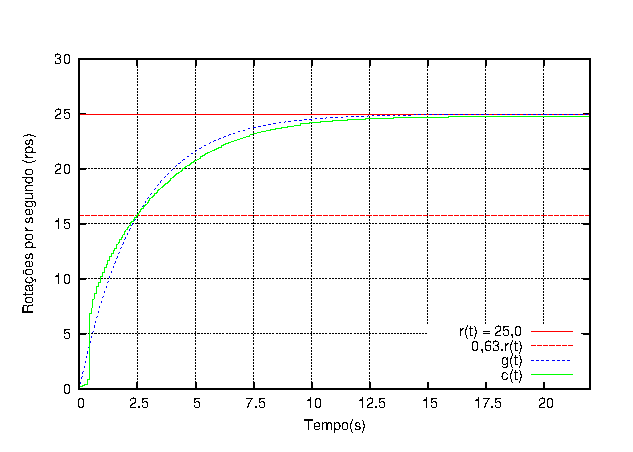
\includegraphics[scale=1.4]{./imagens/acaoMalhaAbertaTau.eps}
\label{fig:acaoMalhaAberTau}

{\small Fonte: Próprio autor}
\end{figure}

A Figura \ref{fig:acaoMalhaAberTau} possui uma linha indicativa que mostra o ponto de intercepção da curva ao valor de 63\% do valor de referência, e empiricamente foi gerado um gráfico com divisões no eixo do Tempo no valor de $\tau = 2,5s $.

Calculando o polo da função:
\begin{equation}
  a = \frac{1}{\tau} = \frac{1}{2,5} = 0,4
\end{equation}

Como $c_{reg} = 25$ e $A$ também é $25$ então na Equação \ref{eq:calcK} $K = a$ e assim temos que:

\begin{equation}
c(t) = \frac{KA}{a}(1-e^{-at}) = \frac{0,4.25}{0,4}(1-e^{-0,4.t}) = 25(1-e^{-0.4.t})
\end{equation}


Aplicando a Transformada de Laplace:

\begin{equation}
  \frac{C(s)}{R(s)} = \frac{K}{s+a} = \frac{0,4}{s+0,4}
\end{equation}


Para a equação no formato canônico tanto o numerador quanto o denominador são divididos pelo próprio valor de $K$. Assim temos que:

\begin{equation}
  \frac{C(s)}{R(s)} = \frac{1}{\tau s+1} = \frac{1}{2,5 s+1}
\end{equation}


Baseado no gráfico mostrado na Figura \ref{fig:acaoMalhaAberTau}, o valor de tempo em que o motor assume a velocidade de referência é aproximadamente $5\tau$, 12,5 s, e como objetivo para uma primeira versão da implementação do controle utilizando LPA$E\tau$ é proposto que o sistema reduza o tempo de alcance da velocidade alvo em um tempo de no máximo $1\tau$, ou seja, $2,5 s$.



\subsubsection{ Qualidade do modelo }

A qualidade do modelo é relativa ao erro aceitável para o sistema estudado. Para o modelo obtido neste estudo foi aplicada o cálculo de Erro Relativo Percentual, e foram feitas análises em trechos diferentes em função da não linearidade inicial apresentada pelo comportamento do motor da planta em estudo.

A equação para o cálculo de Erro Relativo Percentual foi:

\begin{equation}
 \% erro = \frac{| \text{\emph{valor real}} -\text{\emph{valor calculado}} |}{\text{\emph{valor real}}} x 100
\end{equation}

Realizando a somatória para o cálculo de erro médio com todas as amostras aquisitadas: 

\begin{equation}
 \% erro = \frac{100}{N} . \sum_{n = 0,00}^{n=22,40} {\frac{| \text{\emph{r[n]}} -\text{\emph{c[n]}} |}{\text{\emph{r[n]}}} } 
\end{equation}


Onde:

\setlength{\parindent}{2cm}
r : valor real; 

c : valor calculado;

n : número da amostra aquisitada;

N : número total de amostras.

Obs.: As aquisições começaram com tempo inicial de 0,00 s até o tempo final de 22,40 segundos, com intervalo de 10 milisegundos entre aquisições, totalizando 2240 amostras.

\setlength{\parindent}{1cm}

%A Tabela \ref{tab:ErroModelo} mostra o erro médio relativo calculado para diferentes intervalos de tempo. O primeiro valor contempla o intervalo completo de tempo amostrado, de 0,00 até 22,40 s com um erro de 10,77\%. Porém devido a não linearidade inicial, ocorre uma distorção bem grande que pode ser visto nos dois outros intervalos, de 0,00 a 0,50 segundos com erro de 364,13\%, completamente não aceitável, mas que após os 50 milisegundos iniciais, o erro médio é de 2.71\%. 

%Considerando que o intervalo inicial não é pertinente ou relevante para análise aqui proposta,
%assumindo um valor inicial de 50 milisegundos e 
%calculando e erro médio, chegou-se ao valor de 2,71\% de erro 
%para todo o restante da aquisição,
%valor este que é considerado otimo para o modelo.

Foi obtido um valor médio de 2,71\% de erro 
para o intervalo de aquisição de 50ms até os 22,40 s, 
que é o fim da aquisição, 
desconsiderando a região transitória não linear 
que ocorre nos instantes iniciais, 
mas que considera-se não relevante para a atual análise, 
inclusive pelo baixo valor de erro no restante do intervalo de comparação.

%\begin{table}[h]
%\centering
%\caption{Erro Relativo Percentual}
%\label{tab:ErroModelo}

%\begin{tabular}{c|c}
%\hline
%Intervalo de amostras  &  erro médio relativo \\ \hline
%\hline
%0,00 a 22,40 s  &   10,77 \% \\ \hline
%0,00 a  0,50 s 	&  364,13 \% \\ \hline
%0,50 a 22,40 s  &    2,71 \% \\ \hline

%\end{tabular}
%\end{table}


De forma mais detalhada, 
foram calculados os erros médios relativos para cada intervalo de 
tempo de um $\tau$, 
e pode-se notar, 
pela Tabela \ref{tab:ErroModeloTau}, 
que o erro de estado estacionário, para o intervalo acima de 5 $\tau$, é menor do que 1\%. 


\begin{table}[h]
\centering
\caption{Erro Relativo Percentual para intervalos determinados por $\tau$ }
\label{tab:ErroModeloTau}

\begin{tabular}{c|c}
\hline
Intervalo de amostras  &  erro médio relativo \\ \hline
\hline
%0 a 1 $\tau$ & 83,40 \% \\ \hline
1 a 2 $\tau$ &  3,16 \% \\ \hline
2 a 3 $\tau$ &  3,38 \% \\ \hline
3 a 4 $\tau$ &  2,00 \% \\ \hline
4 a 5 $\tau$ &  2,29 \% \\ \hline
$>$ 5 $\tau$ &  0,82 \% \\ \hline
\end{tabular}

{\vspace{0.2cm} \small Fonte: Próprio autor}
\end{table}

%O intervalo inicial, de 0 a 1$\tau$ apresenta um grande erro, devido a não linearidade já comentada anteriormente, que ocorre nos primeiros 50 ms. 

Desconsiderando a região transitória não linear 
que ocorre nos instantes iniciais do movimento do eixo do motor, 
o intervalo de maior erro é de 3,38\%, 
conforme mostrado na Tabela \ref{tab:ErroModeloTau},
ressaltando ainda que no regime estacionário 
o erro é menor do que 1\%.
Assim, considera-se que o modelo utilizado é bom e representa razoavelmente bem o sistema físico real.






\subsection{Requisitos de desempenho do sistema}


Os principais e mais comuns requisitos de desempenho dos sistemas são:

\begin{itemize}
\item Velocidade de resposta:
\item Presença ou não de oscilações na estabilização:
\item Erro de regime estacionário: é a exatidão da resposta do sistema em relação ao valor desejado, assume-se um valor aceitável para o sistema, nesse caso não crítico, de 5\%.
\end{itemize}


\chapter[Resultados Preliminares]{4. Resultados Preliminares}



\section{ Construção de um sistema físico para controle }

 O sistema físico, ou protótipo, foi desenvolvido utilizando a placa de desenvolvimento da Texas Instruments, modelo $Tiva^{TM}$ TM4C123GH6PM, drive para acionamento do motor utilizando PWM, motor DC acoplado a um CD, com uma etiqueta, Figura \ref{fig:discoSensor}, para acionar o sensor óptico e servir de indicador para contagem de giros do motor. Fonte de alimentação chaveada de 12V 10W. A maior parte do sistema pode ser visto na Figura \ref{fig:discoSensorGeral} .



\begin{figure}[!htb]
\center
\caption{Visão geral do sistema }
\subfloat[]{
	\label{fig:discoSensor}
	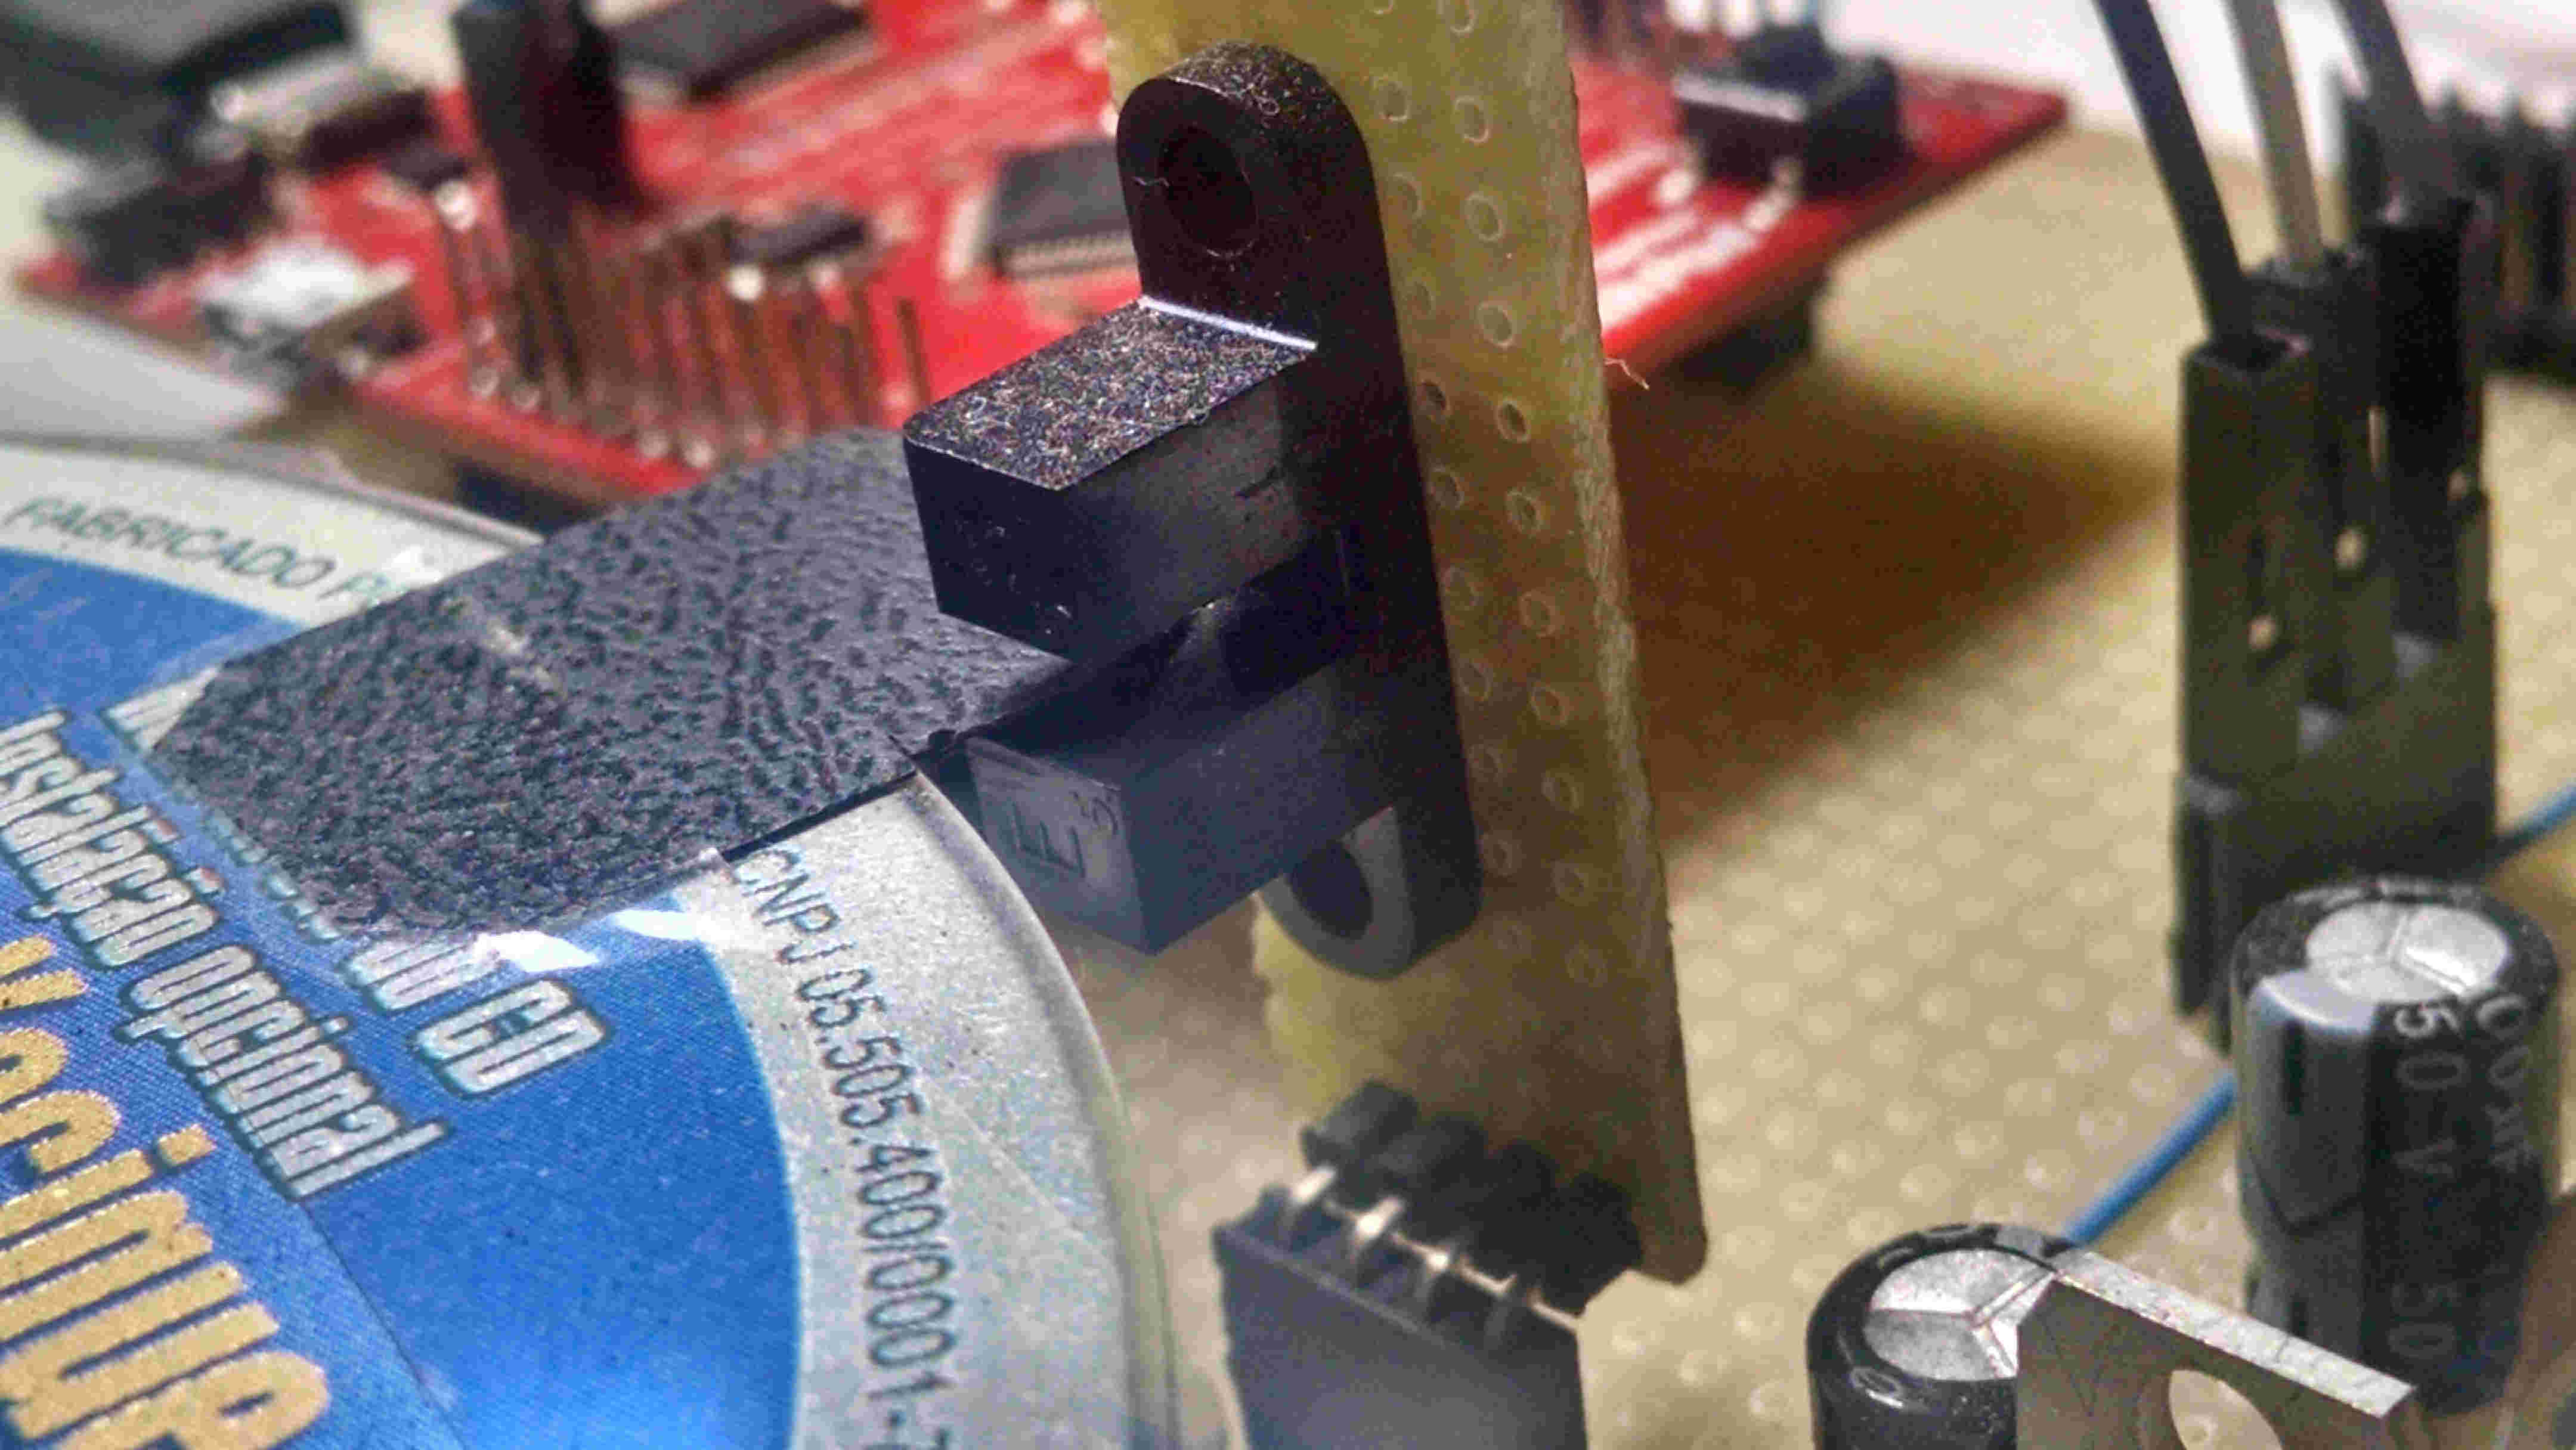
\includegraphics[scale=0.07, angle=0, clip=true, trim=300 200 1200 200]{./imagens/discoSensor.jpg}
	}
\subfloat[]{ 
	\label{fig:discoSensorGeral} 
	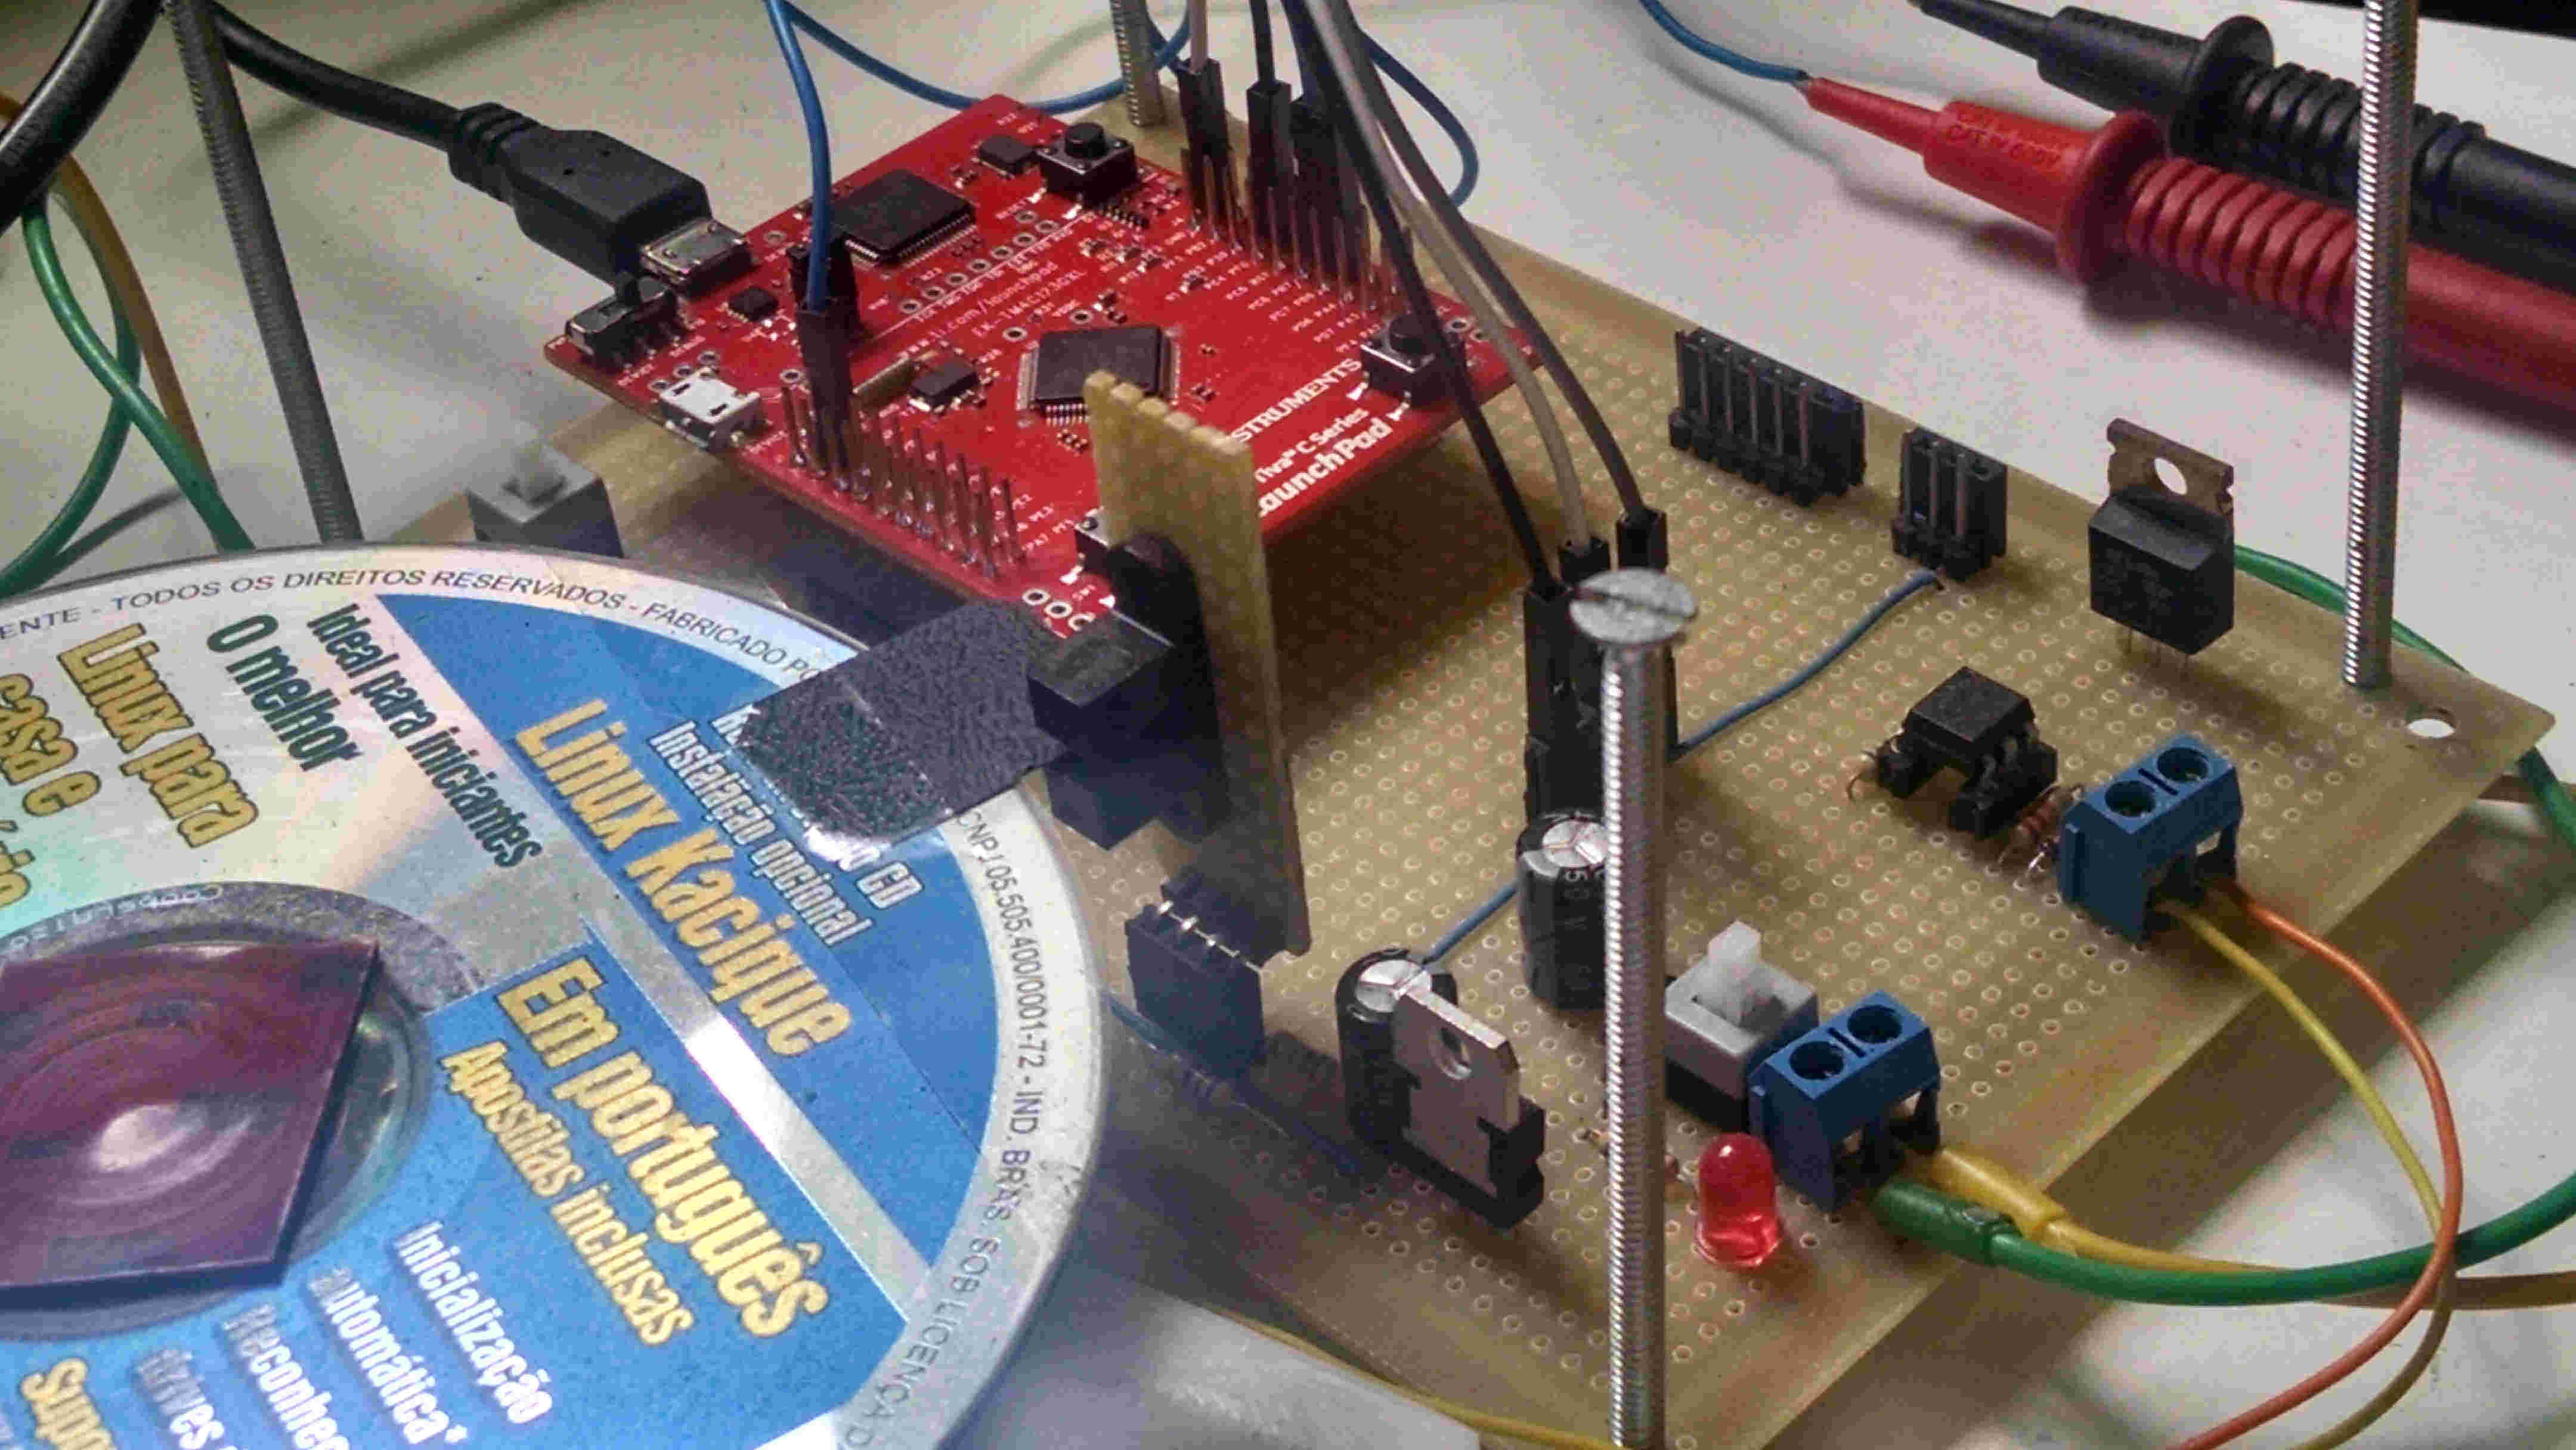
\includegraphics[scale=0.07, angle=0, clip=true, trim=300 200 400 200]{./imagens/discoSensorGeral.jpg} 
	}

{\small Figure: Próprio autor}
\end{figure}


\section{ Obtenção de um modelo do processo }

Para melhor compreensão dos modelos dinâmicos dos sistemas, é utilizado o Diagrama de blocos do comportamento do sistema em malha aberta, conforme Figura \ref{fig:AcaoMalhaAberta}\cite{Ogata}.


\begin{comment}


\begin{figure}[!htb]
\centering
\caption{ Diagrama de blocos de sistema de controle em malha aberta}
\begin{tikzpicture}[scale=0.85]
%\draw [lightgray](0,0) grid (15,2);
\draw (0,1) -- (3,1);
\draw [black, thick](3,0) rectangle (6, 2) ; 
\draw (6,1) -- (9,1);
\draw [black, thick](9,0) rectangle (12, 2) ; 
\draw (12,1) -- (15,1);

\draw [fill]( 3,1) -- ( 2.8, 1.1) -- ( 2.8,0.9) -- ( 3,1);
\draw [fill]( 9,1) -- ( 8.8, 1.1) -- ( 8.8,0.9) -- ( 9,1);
\draw [fill](15,1) -- (14.8, 1.1) -- (14.8,0.9) -- (15,1);

\node at ( 4.5, 1){Controlador};
\node at (10.5, 1){Planta};
\node [above] at ( 1.5,1){Valor de};
\node [below] at ( 1.5,1){Referência};
\node [above] at ( 7.5,1){Variável};
\node [below] at ( 7.5,1){Manipulada};
\node [above] at (13.5,1){Variável};
\node [below] at (13.5,1){Controlada};
\end{tikzpicture}
\label{fig:malhaAberta}

{\small Fonte: \cite{Ogata}}
\end{figure}

\end{comment}

Utilizando variáveis para cada elemento do Diagrama de blocos, de forma a representá-los nas equações, temos então que:



\begin{figure}[!htb]
\centering
\caption{ Sistema de controle em malha aberta}
\begin{tikzpicture}[scale=0.85]
%\draw [lightgray](0,0) grid (15,2);
\draw (0,1) -- (3,1);
\draw [black, thick](3,0) rectangle (6, 2) ; 
\draw (6,1) -- (9,1);
\draw [black, thick](9,0) rectangle (12, 2) ; 
\draw (12,1) -- (15,1);

\draw [fill]( 3,1) -- ( 2.8, 1.1) -- ( 2.8,0.9) -- ( 3,1);
\draw [fill]( 9,1) -- ( 8.8, 1.1) -- ( 8.8,0.9) -- ( 9,1);
\draw [fill](15,1) -- (14.8, 1.1) -- (14.8,0.9) -- (15,1);

\node at ( 4.5, 1.4){Controlador};
\node at ( 4.5, 0.6){f(t)};
\node at (10.5, 1.4){Planta};
\node at (10.5, 0.6){g(t)};
\node [above] at ( 1.5,1){r(t)};
\node [above] at ( 7.5,1){u(t)};
\node [above] at (13.5,1){c(t)};
\end{tikzpicture}
\label{fig:AcaoMalhaAberta}

{\small Fonte: Próprio autor}
\end{figure}


Onde: 

%\begin{itemize}
%\item 
\hspace{1cm} $r(t)$: Valor de Referência em rotações por segundo [rps];

%\item 
$\hspace{1cm} f(t)$: Controlador que converte rps em \% PWM para acionar o motor;

%\item 
$\hspace{1cm} u(t)$: Variável Manipulada é o valor percentual do PWM;

%\item 
$\hspace{1cm} g(t)$: Planta ou Processo formado pelo motor DC com o disco acoplado no eixo;

%\item 
$\hspace{1cm}  c(t)$: Variável Controlada é a velocidade de rotação do eixo em rps.

%\end{itemize}



O sistema físico aqui estudado possui comportamento exponencial que pode ser descrito pela equação \ref{eq:ftSistOrdem1}. 






\begin{equation}
	 \frac{d c(t)}{dt} + c(t) = r(t) \rightarrow  \mathscr{L} \to \frac{C(s)}{R(s)} = \frac{K}{s + a} 
\label{eq:ftSistOrdem1}
\end{equation}

Onde:

\setlength{\parindent}{2cm}

$t$ : tempo,$ r(t) = 0$ , para t $<$ 0;

$\mathscr{L}$ : Operador de Laplace;

$c(t)$ : Variável controlada no domínio do tempo;

$C(s)$ : Variável controlada no domínio da frequência;

$r(t)$ : Valor de referência (\emph{setpoint}) no domínio do tempo;

$R(s)$ : Valor de referência (\emph{setpoint}) no domínio da frequência.

$K$ : Constante de proporcionalidade;

$s$ : Variável complexa de Laplace;

$a$ : Polo da função.
\setlength{\parindent}{1cm}



Sendo assim, para um estímulo de entrada do tipo \textbf{degrau}, com amplitude \textbf{A}, temos $ R(s) = \frac{A}{s}$ e aplicando a Transformada Inversa de Laplace:

\begin{equation}
C(s) = \frac{K}{s+a} \frac{A}{s} \rightarrow \mathscr{L}^{-1} \to c(t) = \frac{K A}{a} (1 - e^{-at})
\label{eq:degrauA}
\end{equation}

A Figura \ref{fig:degrauA} mostra um sinal do tipo degrau com amplitude \textbf{A} aplicado ao sistema de teste, que responde conforme um sistema de primeira ordem como mostrado na Figura \ref{fig:cRegime}. 


%A partir de um determinado instante de tempo, entra em regime constante ($c_{reg}$), alcançando o valor de referência dado pelo degrau de amplitude A. Assim quando $ t \rightarrow \infty $  então $ c_{reg} \rightarrow A $:




\begin{figure}[!htb]
\centering
\caption{Sistema de Primeira Ordem}
\subfloat[Sinal de entrada tipo degrau com amplitude A]{\label{fig:degrauA}
\begin{tikzpicture}[scale=0.75]
\draw [lightgray, dashed](0,0) grid (8.8,5.8);
\draw [->] (0,0) -- (9,0);
\draw [fill] (0,6.2) -- (-0.1, 5.8) -- (0.1,5.8) -- (0,6.2);
\draw [->] (0,0) -- (0,6);
\draw [fill] (9.2,0) -- (8.8,0.1) -- (8.8,-0.1)--(9.2,0.0);
\node at (9.0,-0.5) {$t$};
\node at (0.2,6.5) {$r(t)$};
\draw [red, ultra thick] (0.0,5.0) -- (9.0,5.0);
\draw [red, ultra thick] (0.0,0.0) -- (0.0,5.0);
\node at (-0.5,5.0)[red]{$A$};
\end{tikzpicture} }
\subfloat[Resposta transitória e regime de acomodação]{\label{fig:cRegime}
\begin{tikzpicture}[scale=0.75]
\draw [lightgray, dashed](0,0) grid (8.8,5.8);
\draw [->] (0,0) -- (9,0);
\draw [fill] (0,6.2) -- (-0.1, 5.8) -- (0.1,5.8) -- (0,6.2);
\draw [->] (0,0) -- (0,6);
\draw [fill] (9.2,0) -- (8.8,0.1) -- (8.8,-0.1)--(9.2,0.0);
\node at (9.0,-0.5) {$t$};
\node at (0.2,6.5) {$c(t)$};
\node at (-0.5,5.0)[blue]{$C_{reg}$};
\draw [blue, ultra thick] (0,0) to [out=85, in=180] (6,5);
\draw [blue, ultra thick] (6,5) -- (9,5);
\end{tikzpicture}}
\label{fig:sistPrimeiraOrdem}

{\small Fonte: Próprio autor}
\end{figure}

%\begin{equation}
%c_{reg} = \lim_{t \rightarrow \infty} \frac{KA}{a}(1-e^{-at}) = \frac{KA}{a}
%\label{eq:cregime}
%\end{equation}



%Aplicando o Teorema do Valor Final pode-se ver que o \emph{$c_{reg}$} estabiliza em um valor constante como mostrado pela Equação \ref{eq:teoremaValorFinal}:

%\begin{equation}
%C_{reg} = \lim_{s \rightarrow 0} sC(s) = \lim_{s \rightarrow 0} s\ \frac{K}{s+a}\frac{A}{s} = \frac{KA}{a}
%\label{eq:teoremaValorFinal}
%\end{equation}



Matematicamente, quanto maior o valor de \emph{t} na Equação \ref{eq:degrauA}, o resultado da exponenencial tende a zero, levando a um resultado que depende apenas das constantes para o valor de referência. 

Tomando $t= \frac{1}{a} = a^{-1} = \tau$ para gerar um valor conhecido em $e^{-at}$, da Equação \ref{eq:degrauA} temos:


\begin{equation}
c(a^-1) = \frac{KA}{a}(1-e^{-(a.a^{-1})}) = \frac{KA}{a}(1-e^{-1}) = \frac{KA}{a}.0,63 = 0,63 . C_{reg}
\end{equation}

A Figura \ref{fig:constTempo} mostra a constante de tempo $\tau$, que é atingida quando o sistema alcança 63\% do seu valor de regime. Como sabemos que $\tau = \frac{1}{a}$, então o polo do sistema, que leva o denominador da Equação \ref{eq:degrauA} a zero, é:

\begin{equation}
a = \frac{1}{\tau}
\end{equation}



\begin{figure}
\centering
\caption{Constante de tempo}
\begin{tikzpicture}[scale=1.0]
\draw [lightgray, dashed](0,0) grid (8.8,5.8);

\draw [->] (0,0) -- (9,0);
\draw [fill] (0,6.2) -- (-0.1, 5.8) -- (0.1,5.8) -- (0,6.2);
\draw [->] (0,0) -- (0,6);
\draw [fill] (9.2,0) -- (8.8,0.1) -- (8.8,-0.1)--(9.2,0.0);

\node at (9.0,-0.5) {$t$};
\node at (0.2,6.5) {$c(t)$};

\node at (-0.5,5.0)[blue]{$C_{reg}$};
\node at (-1,5.0*0.63)[purple]{$0,63.c_{reg}$};
\draw [purple, ultra thick, dashed] (0.0,5.0*0.63) -- (1.45,5.0*0.63)
						   -- (1.45,0.0);
\draw [blue, ultra thick] (0,0) to [out=85, in=180] (6,5);
\draw [blue, ultra thick] (6,5) -- (9,5);

\draw [<->] (0.0,-0.4) -- (1.45,-0.4); 
\node at (1.45/2,-0.7){$\tau$};

\end{tikzpicture}
\label{fig:constTempo}

{\small Fonte: Próprio autor}
\end{figure}

Portanto:

\begin{equation}
K = \frac{ac_{reg}}{A}
\label{eq:calcK}
\end{equation}

%\begin{tikzpicture}
%\begin{axis}
%\addplot[title=Gráfico de uma função, 
%	xlabel = {$x$}, ylabel={$y$},
% 	red!70!blue, very thick, samples=200,
%	domain=-3:3]{x/(x^4-3*x^2+4)};
%\end{axis}
%\end{tikzpicture}



%\begin{figure}[!htb]
%\center	
%\includegraphics[scale=1.2]{./imagens/ftMalhaAberta.eps} 
%\label{fig:ftMalhaAberta} 
%\caption{ Função de Transferência empírica da planta}
%\end{figure}





A Figura \ref{fig:AcaoMalhaAberta} mostra um sinal do tipo degrau aplicado como referência no valor de \emph{25 rps}, a curva de comportamento real medida empiricamente e a curva aproximada calculada pelo método determinístico como segue:

\begin{figure}[!htb]
\caption{Ação de Controle em Malha Aberta}
\center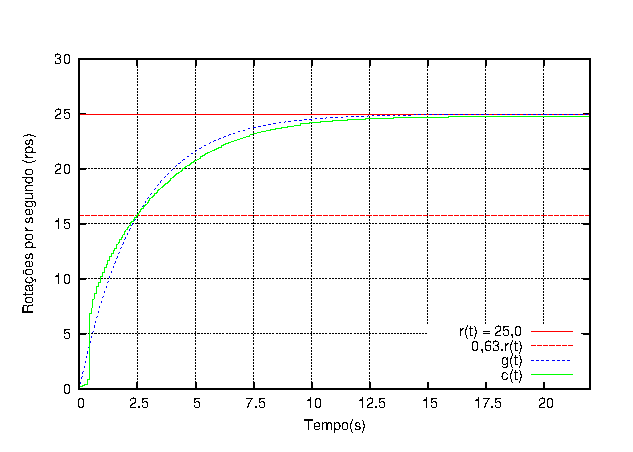
\includegraphics[scale=1.4]{./imagens/acaoMalhaAbertaTau.eps}
\label{fig:acaoMalhaAberTau}

{\small Fonte: Próprio autor}
\end{figure}

A Figura \ref{fig:acaoMalhaAberTau} possui uma linha indicativa que mostra o ponto de intercepção da curva ao valor de 63\% do valor de referência, e empiricamente foi gerado um gráfico com divisões no eixo do Tempo no valor de $\tau = 2,5s $.

Calculando o polo da função:
\begin{equation}
  a = \frac{1}{\tau} = \frac{1}{2,5} = 0,4
\end{equation}

Como $c_{reg} = 25$ e $A$ também é $25$ então na Equação \ref{eq:calcK} $K = a$ e assim temos que:

\begin{equation}
c(t) = \frac{KA}{a}(1-e^{-at}) = \frac{0,4.25}{0,4}(1-e^{-0,4.t}) = 25(1-e^{-0.4.t})
\end{equation}


Aplicando a Transformada de Laplace:

\begin{equation}
  \frac{C(s)}{R(s)} = \frac{K}{s+a} = \frac{0,4}{s+0,4}
\end{equation}


Para a equação no formato canônico tanto o numerador quanto o denominador são divididos pelo próprio valor de $K$. Assim temos que:

\begin{equation}
  \frac{C(s)}{R(s)} = \frac{1}{\tau s+1} = \frac{1}{2,5 s+1}
\end{equation}


Baseado no gráfico mostrado na Figura \ref{fig:acaoMalhaAberTau}, o valor de tempo em que o motor assume a velocidade de referência é aproximadamente $5\tau$, 12,5 s, e como objetivo para uma primeira versão da implementação do controle utilizando LPA2v é proposto que o sistema reduza o tempo de alcance da velocidade alvo em um tempo de no máximo $1\tau$, ou seja, $2,5 s$.


\subsection{ Qualidade do modelo }

A qualidade do modelo é relativa ao erro aceitável para o sistema estudado. Para o modelo obtido neste estudo foi aplicada o cálculo de Erro Relativo Percentual, e foram feitas análises em trechos diferentes em função da não linearidade inicial apresentada pelo comportamento do motor da planta em estudo.

A equação para o cálculo de Erro Relativo Percentual foi:

\begin{equation}
 \% erro = \frac{| \text{\emph{valor real}} -\text{\emph{valor calculado}} |}{\text{\emph{valor real}}} x 100
\end{equation}

Realizando a somatória para o cálculo de erro médio com todas as amostras aquisitadas: 

\begin{equation}
 \% erro = \frac{100}{N} . \sum_{n = 0,00}^{n=22,40} {\frac{| \text{\emph{r[n]}} -\text{\emph{c[n]}} |}{\text{\emph{r[n]}}} } 
\end{equation}


Onde:

\setlength{\parindent}{2cm}
r : valor real; 

c : valor calculado;

n : número da amostra aquisitada;

N : número total de amostras.

Obs.: As aquisições começaram com tempo inicial de 0,00 s até o tempo final de 22,40 segundos, com intervalo de 10 milisegundos entre aquisições, totalizando 2240 amostras.

\setlength{\parindent}{1cm}

%A Tabela \ref{tab:ErroModelo} mostra o erro médio relativo calculado para diferentes intervalos de tempo. O primeiro valor contempla o intervalo completo de tempo amostrado, de 0,00 até 22,40 s com um erro de 10,77\%. Porém devido a não linearidade inicial, ocorre uma distorção bem grande que pode ser visto nos dois outros intervalos, de 0,00 a 0,50 segundos com erro de 364,13\%, completamente não aceitável, mas que após os 50 milisegundos iniciais, o erro médio é de 2.71\%. 

%Considerando que o intervalo inicial não é pertinente ou relevante para análise aqui proposta,
%assumindo um valor inicial de 50 milisegundos e 
%calculando e erro médio, chegou-se ao valor de 2,71\% de erro 
%para todo o restante da aquisição,
%valor este que é considerado otimo para o modelo.

Foi obtido um valor médio de 2,71\% de erro 
para o intervalo de aquisição de 50ms até os 22,40 s, 
que é o fim da aquisição, 
desconsiderando a região transitória não linear 
que ocorre nos instantes iniciais, 
mas que considera-se não relevante para a atual análise, 
inclusive pelo baixo valor de erro no restante do intervalo de comparação.

%\begin{table}[h]
%\centering
%\caption{Erro Relativo Percentual}
%\label{tab:ErroModelo}

%\begin{tabular}{c|c}
%\hline
%Intervalo de amostras  &  erro médio relativo \\ \hline
%\hline
%0,00 a 22,40 s  &   10,77 \% \\ \hline
%0,00 a  0,50 s 	&  364,13 \% \\ \hline
%0,50 a 22,40 s  &    2,71 \% \\ \hline

%\end{tabular}
%\end{table}


De forma mais detalhada, 
foram calculados os erros médios relativos para cada intervalo de 
tempo de um $\tau$, 
e pode-se notar, 
pela Tabela \ref{tab:ErroModeloTau}, 
que o erro de estado estacionário, para o intervalo acima de 5 $\tau$, é menor do que 1\%. 


\begin{table}[h]
\centering
\caption{Erro Relativo Percentual para intervalos determinados por $\tau$ }
\label{tab:ErroModeloTau}

\begin{tabular}{c|c}
\hline
Intervalo de amostras  &  erro médio relativo \\ \hline
\hline
%0 a 1 $\tau$ & 83,40 \% \\ \hline
1 a 2 $\tau$ &  3,16 \% \\ \hline
2 a 3 $\tau$ &  3,38 \% \\ \hline
3 a 4 $\tau$ &  2,00 \% \\ \hline
4 a 5 $\tau$ &  2,29 \% \\ \hline
$>$ 5 $\tau$ &  0,82 \% \\ \hline
\end{tabular}

{\vspace{0.2cm} \small Fonte: Próprio autor}
\end{table}

%O intervalo inicial, de 0 a 1$\tau$ apresenta um grande erro, devido a não linearidade já comentada anteriormente, que ocorre nos primeiros 50 ms. 

Desconsiderando a região transitória não linear 
que ocorre nos instantes iniciais do movimento do eixo do motor, 
o intervalo de maior erro é de 3,38\%, 
conforme mostrado na Tabela \ref{tab:ErroModeloTau},
ressaltando ainda que no regime estacionário 
o erro é menor do que 1\%.
Assim, considera-se que o modelo utilizado é bom e representa razoavelmente bem o sistema físico real.





\section{Resultados}

O processo de implementação da LPA2v como parte do núcleo do controlador 
produziu algumas tentativas sendo que segue aquela de melhor resultado, 
não esgotando as formas e tentativas que poderão se seguir 
no decorrer da pesquisa.


%%%%%%%%%%%%%%%%%%%%%%%%%%%%%%%%%%%%%%%%%%%%%%%%%%
%%%%%%%%%%%%%%%%%%%%%%%%%%%%%%%%%%%%%%%%%%%%%%%%%%
%%%%%%%%%%%%%%%%%%%%%%%%%%%%%%%%%%%%%%%%%%%%%%%%%%
%%%%%%%%%%%%%%%%%%%%%%%%%%%%%%%%%%%%%%%%%%%%%%%%%%
\begin{comment}
O código da Figura \ref{fig:codigoGcGct} mostra 
a implementação da função que calcula os graus de Certeza e Contradição 
tendo como parâmetro de entrada dois graus de evidência favoráveis.

A LPA2v foi codificada utilizando variáveis do tipo ponto flutuante 
de forma a trabalhar com os seus parâmetros da mesma forma como a lógica é 
proposta e analisada conceitualmente, por isso, inclusive, 
a utilização de um microcontrolador com um módulo dedicado 
ao cálculo utilizando variáveis desse tipo. 


\begin{figure}[!htb]
\centering
\caption{Código de função que calcula os graus de Certeza e Contradição utilizando LPA2v}
\begin{minipage}{0.9\linewidth}
\begin{lstlisting}
float Gc, Gct;

void LPA2v( float u0, float u1 )
{
  float l0, l1;
  l0 = 1.0 - u0;
  l1 = 1.0 - u1;

  Gc  = u0 - l1;
  Gct = (u0 + l1) - 1.0;
}
\end{lstlisting}
\end{minipage}
\label{fig:codigoGcGct}

{\small Fonte: Próprio autor}
\end{figure}

A função \texttt{LPA2v} possui como parâmetros de entrada 
dois graus de certeza, simplesmente para facilitar o raciocínio,
sendo que os respectivos graus de inceteza 
são declarados como variáveis locais na linha 5 e calculados nas linhas 6 e 7.

As linhas 9 e 10 apresentam o cálculo dos graus de Certeza e Contradição, 
sendo as respectivas variáveis declaradas como globais, linha 1, 
por serem elas utilizadas em outras funções.






\begin{figure}[!htb]
\centering
\caption{Código de função do controlador utilizando a LPA2v}
\begin{minipage}{0.9\linewidth}
\lstset{firstnumber=12}
\begin{lstlisting}
#define KLP 	10
long controlador( long setpoint, long max, long sensor )
{
  float aux, rT, hT;
  long uT;

  rT = (float) setpoint / (float) max;
  hT = (float) sensor   / (float) max;

  if( rT > 1.0 )
    rT = 1.0;
  if( hT > 1.0 )
    hT = 1.0;
  
  aux = (rT * 100.0);

  LPA2v( rT, hT );
  
  uT = (long)(aux + aux * Gct * KLP);
  if( uT > 99 )
    uT = 99;
  if( uT < 0 ) 
    uT = 0;
  return( uT );
}

\end{lstlisting}
\end{minipage}
\label{fig:codigoControladorLPA2v}

{\small Fonte: Próprio autor}
\end{figure}

\end{comment}

%%%%%%%%%%%%%%%%%%%%%%%%%%%%%%%%%%%%%%%%%%%%%%%%%%
%%%%%%%%%%%%%%%%%%%%%%%%%%%%%%%%%%%%%%%%%%%%%%%%%%
%%%%%%%%%%%%%%%%%%%%%%%%%%%%%%%%%%%%%%%%%%%%%%%%%%
%%%%%%%%%%%%%%%%%%%%%%%%%%%%%%%%%%%%%%%%%%%%%%%%%%

A Figura \ref{fig:diagramaBlocosLPA2v} mostra 
o diagrama de blocos da implementação da 
LPA2v inserida na malha de controle. 

\begin{figure}[!h]
\centering
\caption{Diagrama de blocos do controle utilizando a LPA2v}
\begin{tikzpicture}[scale=1.0]
\tikzset{ >=latex, inner sep=0pt, outer sep=0pt,  }

%\draw [lightgray, dashed](0,0) grid (15,7);

%%% Blocos 

% K normalização rps -> 0..1
\node [fill=black, circle] (KSP0) at (1,6.5) { };
\node [fill=black, circle] (KSP1) at (2,5.5) { };
\draw[thick] (KSP0) rectangle (KSP1);
\fill[white, nearly transparent] (KSP0) rectangle (KSP1);
\node [fill=black, circle] (KSPin)  at (1.0,6.0) { }; 
\node [fill=black, circle] (KSPout) at (2.0,6.0) { }; 
\node (Kn1) at (1.5,6.0) {$K_n$};

% K normalização  0..1 --> %PWM
\node [fill=black, circle] (KPWM0) at (4,6.5) { };
\node [fill=black, circle] (KPWM1) at (5,5.5) { };
\draw[thick] (KPWM0) rectangle (KPWM1);
\fill[white, nearly transparent] (KPWM0) rectangle (KPWM1);
\node [fill=black, circle] (KPWMin)  at (4.0,6.0) { };
\node [fill=black, circle] (KPWMout) at (5.0,6.0) { };
\node (K100) at (4.5,6.0) {$K_{\%}$};

% Planta
\node [fill=black, circle] (GT0) at (13,6.5) { };
\node [fill=black, circle] (GT1) at (14,5.5) { };
\draw[thick] (GT0) rectangle (GT1);
\fill[white, nearly transparent] (GT0) rectangle (GT1);
\node [fill=black, circle] (GTin)  at (13.0,6.0) { };
\node [fill=black, circle] (GTout) at (14.0,6.0) { };
\node (planta) at (13.5,6.0) {$g(t)$};

% Saturação
\node [fill=black, circle] (SAT0) at (11,6.5) { };
\node [fill=black, circle] (SAT1) at (12,5.5) { };
\draw[thick] (SAT0) rectangle (SAT1);
\fill[white, nearly transparent] (SAT0) rectangle (SAT1);
\node [fill=black, circle] (SATin)  at (11.0,6.0) { };
\node [fill=black, circle] (SATout) at (12.0,6.0) { };
\draw [thick] (11.2,5.7) -- (11.4,5.7) -- (11.6,6.3) -- (11.8,6.3);
\draw [gray, thick] (11.2,6.0) -- (11.8,6.0);
\draw [gray, thick] (11.5,5.7) -- (11.5,6.3);

% Multiplicacao
\node [fill=black, circle] (MUL0) at (8,4.5) { };
\node [fill=black, circle] (MUL1) at (9,2.5) { };
\draw[thick] (MUL0) rectangle (MUL1);
\fill[white, nearly transparent] (MUL0) rectangle (MUL1);
\node [fill=black, circle] (MULin0) at (8.0,4.0) { };
\node [fill=black, circle] (MULin1) at (8.0,3.0) { };
\node [fill=black, circle] (MULout) at (9.0,3.5) { };
\node (multi) at (8.5,3.5) {$x$};

% Klp
\node [fill=black, circle] (KLP0) at (6,3.5) { };
\node [fill=black, circle] (KLP1) at (7,2.5) { };
\draw[thick] (KLP0) rectangle (KLP1);
\fill[white, nearly transparent] (KLP0) rectangle (KLP1);
\node [fill=black, circle] (KLPin)  at (6.0,3.0) { };
\node [fill=black, circle] (KLPout) at (7.0,3.0) { };
\node (KLP) at (6.5,3.0) {$K_{LP}$};

% Sensor
\node [fill=black, circle] (KS0) at (6,1.5) { };
\node [fill=black, circle] (KS1) at (7,0.5) { };
\draw[thick] (KS0) rectangle (KS1);
\fill[white, nearly transparent] (KS0) rectangle (KS1);
\node [fill=black, circle] (KSin)  at (7.0,1.0) { };
\node [fill=black, circle] (KSout) at (6.0,1.0) { };
\node (Kn2) at (6.5,1.0) {$K_n$};

% LPA2v
\node [fill=black, circle] (LPA0) at (3,4.5) { };
\node [fill=black, circle] (LPA1) at (5,2.5) { };
\draw[thick] (LPA0) rectangle (LPA1);
\fill[white, nearly transparent] (LPA0) rectangle (LPA1);
\node [fill=black, circle] (LPAu0) at (3.0,4.0) { };
\node [fill=black, circle] (LPAu1) at (3.0,3.0) { };
\node [fill=black, circle] (LPAgc)  at (5.0,4.0) { };
\node [fill=black, circle] (LPAgct) at (5.0,3.0) { };
\draw [thick] (4.0,4.5) -- (5.0,3.5) -- (4.0,2.5) -- (3.0,3.5) -- (4.0,4.5);
\node (LPA2v) at (4.0,3.5) {$LPA2v$};
\draw [thick] (LPAgc) -- (5.3,4.0);
\node (LPA2vu0)  at (2.0,4.1) {$\mu _0$};
\node (LPA2vu1)  at (2.0,3.1) {$\mu _1$};
\node (LPA2vGc)  at (5.3,4.3) {$G_c$};
\node (LPA2vGct) at (5.3,3.3) {$G_{ct}$};


% Somador
\node [fill=black, circle] (SUM) at (9.5,6.0) { };
\filldraw[fill=white,thick] (SUM) circle (5mm);
\node [fill=black, circle] (SUMin0) at ( 9.0,6.0) { };
\node [fill=black, circle] (SUMin1) at ( 9.5,5.5) { };
\node [fill=black, circle] (SUMout) at (10.0,6.0) { };
\node (Sum0) at (9.2,6.0) {$+$};
\node (Sum1) at (9.5,5.7) {$+$};



%%% Linhas 

% set point
\draw [->, thick] (0.0,6.0) -- (KSPin);
\node (rt) at (0.5,6.3) {$r(t)$};

% setpoint -> normalização %PWM
\draw [->, thick] (KSPout) -- (KPWMin);

% normalização %PWM -> SUM
\draw [->, thick] (KPWMout) -- (SUMin0);

% SUM -> Saturação
\draw [->, thick] (SUMout) -- (SATin);

% Saturação -> GT
\draw [->, thick] (SATout) -- (GTin);

% GT -> fim
\draw [->, thick] (GTout) -- (15,6);
\node (ct) at (14.5,6.3) {$c(t)$};

% LPA2v Gct -> KLP
\draw [->, thick] (LPAgct) -- (KLPin);

% KLP -> MULin1
\draw [->, thick] (KLPout) -- (MULin1);

% normalização 0..1 -> LPA2v u0
\draw [->, thick] (2.5,6.0) -- (2.5,4.0) -- (LPAu0);

% normalização %PWM -> MULT in0
\draw [->, thick] (7.5,6.0) -- (7.5,4.0) -- (MULin0);

% MULT out -> SUM in1
\draw [->, thick] (MULout) -- (9.5,3.5) -- (SUMin1);

% Fim -> sensor
\draw [->, thick] (14.5,6.0) -- (14.5,1.0) -- (KSin);

% Sensor -> LPA u2
\draw [->, thick] (KSout) -- (2.5,1.0) -- (2.5,3.0) --(LPAu1);

\end{tikzpicture}
\label{fig:diagramaBlocosLPA2v}

{\vspace{0.2cm} \small Fonte: Próprio autor}
\end{figure}

Temos então a descrição dos blocos :

\begin{itemize}
  \item $K_n$: Bloco de normalização da grandeza de velocidade de giro do motor em rotações por segundo para o intervalo fechado entre 0,0 e 1,0. 
São dois bloco, sendo um para o parâmetro de referência, 
ou \emph{setpoint}, e o outro para o sinal do sensor que efetua a 
leitura diretamente na planta de processo;

  \item $K_{\%}$: Normaliza o valor em um intervalo fechado de 0,0 a 1,0 para um intervalo de 0 a 100 correspondente ao parâmetro do acionamento por PWM;

  \item $LPA2v$: Calcula os graus de Certeza e Contradição 
de acordo com os parâmetros de entrada, 
que são os graus de evidência favorável $\mu _0$ e $\mu _1$ e são
respectivamente referentes ao valor desejado e 
ao valor real lido diretamente na planta;

  \item $K_{LP}$: Coeficiente de ganho proporcional do grau de contradição;

  \item $x$: Bloco multiplicador;

  \item $g(t)$: Planta do sistema;

  \item $Soma$: Bloco somador;

  \item \emph{Saturação}: Bloco limitador, impede o valor do PWM ultrapassar seu valor máximo de 100\%. 
\end{itemize}



Para implementação do controlador foram realizados alguns testes 
para verificar a velocidade máxima que o motor alcança, 
chegando ao valor de 85 rotações por segundo (rps), com isso, 
foi possível ajustar o bloco $K_n$ para $\frac{1}{85}$, 
e sabe-se que o limite máximo para entrada em $r(t)$ é 85 e o mínimo é 0.

O bloco $K_\%$ é apenas um fator multiplicador com valor 100.

O bloco da $LPA2v$ apresenta a seguinte proposição:

\emph{ P: O eixo do motor apresenta rotação igual ao valor de referência.}

Para tal proposição, 
são utilizados dois especialistas: 
$\mu _0$ é o grau de crença que refere-se ao valor desejado, 
e corresponde ao valor teórico para acionamento do PWM;
e $\mu _1$, que é o grau de crença com que o motor 
atinge a velocidade de giro desejada, 
é o valor utilizado como realimentação do sistema.

O bloco LPA2v calcula os graus de descrença das respectivas entradas:

\begin{equation}
\lambda _0 = 1- \mu _0   \hspace{1cm}   \lambda _1 = 1 - \mu_1 
\end{equation}

Para o cálculo dos graus de Certeza e Contradição são utilizados:

\begin{equation}
P _{(\mu_0, \lambda_1)}
\end{equation}


Os resultados da ação de controle utilizando a LPA2v são mostrados na 
Figura \ref{fig:acaoLPA2v}, onde pode-se ver que 
para um $K_{LP}$ variando de 4 até 10, 
o sistema apresenta comportamento que atende aos requisitos de desempenho,
pois o valor de regime entra na janela formada pelo erro de $5\%$ referente
ao valor desejado em um tempo menor do que um $\tau$, ou seja, 2,5s.
Mesmo o sobressinal gerado com $K_{LP} = 10$, 
não chega a ultrapassar o valor limite máximo de erro. 


\begin{figure}[!htb]
\caption{Ação de controle utilizando LPA2v}
\vspace{-1cm}\center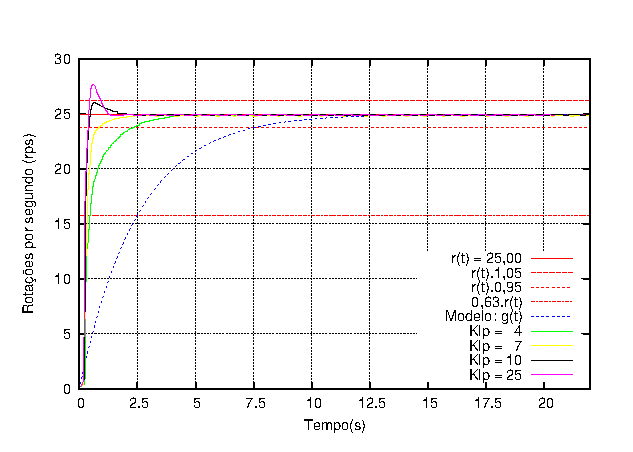
\includegraphics[scale=1.6]{./imagens/klpAll.eps}
\label{fig:acaoLPA2v}

{\small Fonte: Próprio autor}
\end{figure}


Em um segundo momento foi gerado um sinal de referência variável,
assumindo valores de patamar diferentes a 
cada intervalo de tempo aproximado de 10s.
A Figura \ref{fig:acaoLPA2vpatam85} mostra 
o sinal de referência junto ao sinal de resposta da planta,
onde nota-se que com um degrau com variação de 25, 
houve um sobressinal, porém para os demais patamares, 
a variação foi menor, e com isso, 
não apresentaram sobressinal. 
Outro ponto notado foi que o erro é cada vez maior quanto maior for o 
valor de desejado, de referência. 



\begin{figure}[!htb]
\caption{Ação de controle utilizando LPA2v para valores alvo variáveis}
\vspace{-1cm}
\center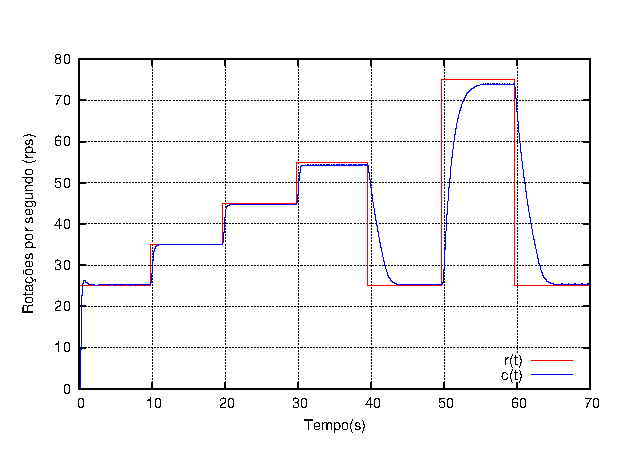
\includegraphics[scale=1.4]{./imagens/patam85.eps}
\label{fig:acaoLPA2vpatam85}

{\small Fonte: Próprio autor}
\end{figure}



Apesar destes detalhes o resultado é tido como muito bom e promissor,
pois possibilitou que a LPA2v fosse testada de forma empírica em um sistema
de controle dinâmico, obtendo uma performance dentro de um padrão mínimo 
estabelecido.





\section{Etapas a serem desenvolvidas}

\begin{itemize}
\item Estudar a LPA2v;
\item Implementar um controlador utilizando LPA2v;
	\begin{itemize}
	\item Estabelecer a configuração do sistema;
	\item Descrever o controlador e parâmetros de ajuste;
	\end{itemize}
\item Otimizar parâmetros e analisar performance;
\end{itemize}





\chapter[Cronograma]{5. Cronograma}
%\chapter{Cronograma}

As atividades a serem desenvolvidas para a 
conclusão e defesa da dissertação de mestrado 
são apresentadas na forma de descrição e na forma de tabela.

A descrição apresenta a série de tarefas 
a serem realizadas após a qualificação, 
sendo cada uma das tarefas denotada como uma entrega 
a ser realizada ao orientador.

O cronograma ajustado para datas de entrega dos fragmentos do trabalho,
 possibilita a visão e o esforço focados na tarefa, 
e foi baseado em metodologias ágeis.


As tarefas são as seguintes:

\begin{enumerate}
  \item \label{LPA2v}	    Entregar o estudo da LPA2v aplicada ao Controle de Sistemas.

A LPA2v possui uma grande diversidade de aplicações, 
e tendo o controle de sistemas 
uma das áreas de pouca ou talvez nenhuma aplicação, 
pois ainda não foi encontrado qualquer artigo que mostrasse seu uso. 
Assim essa tarefa consiste em se aprofundar nas pesquisas 
da utilização da LPA2v em sistemas de controle de processos. 

  \item \label{controlar}   Entregar a implementação de um controlador utilizando LPA2v.

Implementar um modelo de controlador, 
baseado no exemplo de aplicação em controle de sistemas
trazido pelo Profº Dr. João Inácio da Silva Filho em sua 
tese de doutorado defendida na Universidade de São Paulo, 
sendo ele um dos precursores da aplicação da LPA2v. 

  \item \label{configurar}  Entregar a configuração do controlador.

Formatar um modelo estabelecendo a configuração do controlador desenvolvido.

  \item \label{descrever}   Entregar a descrição do controlador e dos parâmetros de ajuste.

Dado o controle utilizando a LPA2v em operação, 
serão descritos os parâmetros de ajuste e a configuração do controlador, 
permitindo uma fácil reprodução para novos ensaios e aplicações.

  \item \label{otimizar1}   Entregar a primeira otimização dos parâmetros e analise da performance.

Primeira etapa de otimização após a descrição do controlador,
onde possíveis alterações podem ser realizadas, 
com o intuito de corrigir conceitos e 
formas de aplicação, ou ainda, 
um refinamento do controlador.

  \item \label{otimizar2}   Entregar a segunda otimização dos parâmetros e analisar a performance do controlador.

Segunda etapa de otimização para pequenos acertos de 
configuração ou decodificação.

  \item \label{entregar}    Entregar a revisão de toda a dissertação.

Revisão geral da dissertação, envolvendo conferência das referências, formatação no padrão estabelecida pela instituição avaliadora, correções ortográficas e gramaticais.

  \item \label{finalizar}   Entregar a dissertação finalizada.

Finalizar a versão para correção do orientador.

  \item \label{corrigir}    Entregar a correção da dissertação.

Após apontamentos do orientador, correção final.

  \item \label{imprimir}    Entregar a impressão da dissertação.

Realizar a impressão de quatro vias da dissertação, sendo três vias a serem  enviadas à banca examinadora e uma para próprio uso.

  \item \label{finalApres}  Entregar a apresentação finalizada.

Baseado na dissertação finalizada, concluir a produção da apresentação.

  \item \label{apresentar}  Apresentar a dissertação.

\end{enumerate}


%\begin{table}[htbp]
\begin{table}[t]
\caption{Cronograma de atividades}
\begin{center}
\resizebox{\textwidth}{!}
{
  \begin{tabular}{c|l|l|l|l|l|l|l|l|l|l|l|l }
  \hline
  \multicolumn{1}{c|}
     {\multirow{2}{*}{Tarefas}} & 
     \multicolumn{2}{c|}{Jul} &
     \multicolumn{2}{|c|}{Ago} &
     \multicolumn{2}{|c|}{Set} & 
     \multicolumn{2}{|c|}{Out} &
     \multicolumn{2}{|c|}{Nov} &
     \multicolumn{2}{|c }{Dez} \\ \cline{2-13}
     \multicolumn{1}{ c|}{} & 12 & 26 & 16 & 30 & 13 & 27 & 11 & 25 & 15 & 29 & 06 & 13 \\ 
  \hline
  \hline
  %\rowcolor[HTML]{EFEFEF}
  \ref{LPA2v} 	  & \cellcolor{lightgray} &&&&&&&&&&&  \\ \hline
  \ref{controlar} && \cellcolor{lightgray} &&&&&&&&&&  \\ \hline
  \ref{configurar}&&& \cellcolor{lightgray} &&&&&&&&&  \\ \hline
  \ref{descrever} &&&& \cellcolor{lightgray} &&&&&&&&  \\ \hline
  \ref{otimizar1} &&&&& \cellcolor{gray} &&&&&&&  \\ \hline
  \ref{otimizar2} &&&&&& \cellcolor{gray} &&&&&&  \\ \hline
  \ref{entregar}  &&&&&&& \cellcolor{darkgray} &&&&&  \\ \hline
  \ref{finalizar} &&&&&&&& \cellcolor{darkgray} &&&&  \\ \hline
  \ref{corrigir}  &&&&&&&&& \cellcolor{darkgray} &&&  \\ \hline
  \ref{imprimir}  &&&&&&&&&& \cellcolor{darkgray} &&  \\ \hline
  \ref{finalApres}&&&&&&&&&& \cellcolor{darkgray} &&  \\ \hline
  \ref{apresentar}&&&&&&&&&&& \cellcolor{black} &  \\ \hline
  \hline
  \end{tabular}
}
\end{center}
\label{tab:cronograma}
\vspace{0.5cm}
\centering
{\small Fonte: Próprio autor}
\end{table}



\chapter[Viabilidade Econômica]{6. Viabilidade Econômica}
Para a efetiva execução da pesquisa, 
dentro das perspectivas propostas e estabelecidas pelo autor, 
sendo  necessária a construção do sistema físico, 
e juntamente com outros recursos,
apresenta-se aqui o aspecto econômico 
referente aos custos envolvidos na viabilização deste trabalho. 
 

\begin{table}[h]
\centering
\caption{Custo dos itens adquiridos para montagem do projeto}
\label{tab:custos}
\begin{tabular}{c|c|c}
\hline
Item  & Descrição  & Valor \\ \hline
\hline
1 & Placa de desenvolvimento modelo Tiva$ ^{TM}$ TM4C123GH6PM & $R\$ 42,00 $ \\ \hline
2 & Placa padrão perfurada 10x15 cm & $R\$ 15,00 $ \\ \hline
3 & Componentes eletrônicos diversos & $R\$20,00$ \\ \hline
4 & Fonte de alimentação & $R\$60,00 $ \\ \hline
\hline
  & Total & $R\$137,00 $ \\ \hline
\hline
\end{tabular}

{\vspace{0.4cm} \small Fonte: Próprio autor}
\end{table}

O item 3 da Tabela \ref{tab:custos} refere-se aos componentes para montagem do circuito de acionamento do motor e como elementos principais pode-se citar: Transistor MOSFET IRF640N, Optoacoplador 4n25, Interruptor óptico HOA0862-T55, capacitores, resistores, diodos, regulador de tensão, conectores. 


Alguns equipamentos ou componentes não geraram custos ao projeto devido a serem itens de uso comum a outras atividades do autor. 

\begin{table}[h]
\centering
\caption{Itens que não geraram custo direto ao projeto}
\label{tab:equipamentos}
\begin{tabular}{c|c}
\hline
Item  & Descrição \\ \hline
\hline
1 & Microcomputador portátil - Notebook \\ \hline
2 & Softwares  \\ \hline
3 & Multímetro \\ \hline
4 & Motor DC \\ \hline
5 & Disco acoplado ao motor \\ \hline
\hline
\end{tabular}

{\vspace{0.4cm} \small Fonte: Próprio autor}
\end{table}

O item 2 da Tabela \ref{tab:equipamentos} 
refere-se aos softwares utilizados em todo o desenvolvimento do trabalho, 
sendo estes ferramentas de uso livre utilizadas previamente pelo autor, 
como sistema operacional GNU/Linux Debian 8(Jessie), 
GNOME Shell, 
Editor de texto e códigos fonte VIM, 
compilador GCC para ARM (arm-none-eabi-gcc), 
GNU Make, 
processador de texto \LaTeX - pdfTEX, 
pacotes geradores de figuras TikZ, PGF e GNU pic(Groff), 
gerador de gráficos GNUPlot, 
teminal de comunicação Minicom e 
gravador LM4Flash.


Todos os custos referentes ao projeto foram custeados pelo próprio autor, em função da natureza e limitação do trabalho proposto.



%%-------------------------------------- Bibliografia
%\printbibliography
%\bibliographystyle{plain}
%\bibliographystyle{abnt-alf}
%\bibliography{bibliografia.bib}

\bibliographystyle{abnt-num}
\bibliography{bibliografia}



%%-------------------------------------- Apendice
%%\appendix
%%\chapter{Titulo do Apendice}

%%-------------------------------------- Anexo
%%\annex
%%\chapter{Titulo do Anexo}



\end{document}




% bibliographystyle tipos
%http://www.cs.stir.ac.uk/~kjt/software/latex/showbst.html

%%%% Estrutura base do arquivo
%%[] http://www.demat.ufma.br/monografia.php <acesso em 12/10/2015>
%%%% Inclusão de pacote de acentuação Francês/Portugues
%%[] https://www.overleaf.com/help/61-how-do-i-do-to-use-letters-with-accents-e-dot-g-in-french-or-portuguese#.Vhwirc8Tr18 <acesso em 12/10/2015 


%http://link.periodicos.capes.gov.br/sfxlcl41?frbrVersion=2&ctx_ver=Z39.88-2004&ctx_enc=info:ofi/enc:UTF-8&ctx_tim=2015-10-27T23%3A55%3A45IST&url_ver=Z39.88-2004&url_ctx_fmt=infofi/fmt:kev:mtx:ctx&rfr_id=info:sid/primo.exlibrisgroup.com:primo3-Article-doaj&rft_val_fmt=info:ofi/fmt:kev:mtx:journal&rft.genre=article&rft.atitle=Implementation+of+PID+and+Fuzzy+PID+controllers+for+Temperature+control+in+CSTR&rft.jtitle=International+Journal+of+Advanced+Research+in+Computer+Science&rft.btitle=&rft.aulast=&rft.auinit=&rft.auinit1=&rft.auinitm=&rft.ausuffix=&rft.au=S.+Srinivasulu+Raju&rft.aucorp=&rft.date=20130501&rft.volume=04&rft.issue=05&rft.part=&rft.quarter=&rft.ssn=&rft.spage=12&rft.epage=&rft.pages=&rft.artnum=&rft.issn=0976-5697&rft.eissn=&rft.isbn=&rft.sici=&rft.coden=&rft_id=info:doi/&rft.object_id=&svc_val_fmt=info:ofi/fmt:kev:mtx:sch_svc&rft.eisbn=&rft_dat=%3Cdoaj%3E01c00f89709d40549e219bbc941a6a0a%3C/doaj%3E%3Cgrp_id%3E7778711627802309381%3C/grp_id%3E%3Coa%3E%3C/oa%3E&rft_id=info:oai/&svc.fulltext=yes&req.language=por

% http://link.periodicos.capes.gov.br/sfxlcl41?frbrVersion=3&ctx_ver=Z39.88-2004&ctx_enc=info:ofi/enc:UTF-8&ctx_tim=2015-10-27T23%3A55%3A45IST&url_ver=Z39.88-2004&url_ctx_fmt=infofi/fmt:kev:mtx:ctx&rfr_id=info:sid/primo.exlibrisgroup.com:primo3-Article-springer_jour&rft_val_fmt=info:ofi/fmt:kev:mtx:&rft.genre=&rft.atitle=Adaptive+fuzzy+tuning+of+PID+controllers&rft.jtitle=Neural+Computing+and+Applications&rft.btitle=&rft.aulast=Esfandyari&rft.auinit=&rft.auinit1=&rft.auinitm=&rft.ausuffix=&rft.au=Esfandyari%2C+Morteza&rft.aucorp=&rft.date=201312&rft.volume=23&rft.issue=1&rft.part=&rft.quarter=&rft.ssn=&rft.spage=19&rft.epage=28&rft.pages=&rft.artnum=&rft.issn=0941-0643&rft.eissn=1433-3058&rft.isbn=&rft.sici=&rft.coden=&rft_id=info:doi/10.1007%2Fs00521-012-1215-8&rft.object_id=&svc_val_fmt=info:ofi/fmt:kev:mtx:sch_svc&rft.eisbn=&rft_dat=%3Cspringer_jour%3E10.1007%2Fs00521-012-1215-8%3C/springer_jour%3E%3Cgrp_id%3E6653138538760267648%3C/grp_id%3E%3Coa%3E%3C/oa%3E&rft_id=info:oai/&svc.fulltext=yes&req.language=por

%http://link.periodicos.capes.gov.br/sfxlcl41?frbrVersion=2&ctx_ver=Z39.88-2004&ctx_enc=info:ofi/enc:UTF-8&ctx_tim=2015-10-27T23%3A55%3A45IST&url_ver=Z39.88-2004&url_ctx_fmt=infofi/fmt:kev:mtx:ctx&rfr_id=info:sid/primo.exlibrisgroup.com:primo3-Article-sciversesciencedirect_elsevier&rft_val_fmt=info:ofi/fmt:kev:mtx:&rft.genre=article&rft.atitle=A+multivariable+predictive+fuzzy+PID+control+system&rft.jtitle=Applied+Soft+Computing+Journal&rft.btitle=&rft.aulast=Savran&rft.auinit=&rft.auinit1=&rft.auinitm=&rft.ausuffix=&rft.au=Savran%2C+Aydogan&rft.aucorp=&rft.date=2012&rft.volume=&rft.issue=&rft.part=&rft.quarter=&rft.ssn=&rft.spage=&rft.epage=&rft.pages=&rft.artnum=&rft.issn=1568-4946&rft.eissn=&rft.isbn=&rft.sici=&rft.coden=&rft_id=info:doi/10.1016%2Fj.asoc.2012.11.021&rft.object_id=&svc_val_fmt=info:ofi/fmt:kev:mtx:sch_svc&rft.eisbn=&rft_dat=%3Csciversesciencedirect_elsevier%3ES1568-4946%2812%2900505-4%3C/sciversesciencedirect_elsevier%3E%3Cgrp_id%3E824269217450252803%3C/grp_id%3E%3Coa%3E%3C/oa%3E&rft_id=info:oai/&svc.fulltext=yes&req.language=por

%http://link.periodicos.capes.gov.br/sfxlcl41?frbrVersion=3&ctx_ver=Z39.88-2004&ctx_enc=info:ofi/enc:UTF-8&ctx_tim=2015-10-27T23%3A55%3A45IST&url_ver=Z39.88-2004&url_ctx_fmt=infofi/fmt:kev:mtx:ctx&rfr_id=info:sid/primo.exlibrisgroup.com:primo3-Article-gale_ofa&rft_val_fmt=info:ofi/fmt:kev:mtx:&rft.genre=article&rft.atitle=A+multivariable+predictive+fuzzy+PID+control+system.&rft.jtitle=Applied+Soft+Computing+Journal&rft.btitle=&rft.aulast=&rft.auinit=&rft.auinit1=&rft.auinitm=&rft.ausuffix=&rft.au=Savran%2C+Aydogan&rft.aucorp=&rft.date=20130501&rft.volume=13&rft.issue=5&rft.part=&rft.quarter=&rft.ssn=&rft.spage=2658&rft.epage=&rft.pages=&rft.artnum=&rft.issn=1568-4946&rft.eissn=&rft.isbn=&rft.sici=&rft.coden=&rft_id=info:doi/&rft.object_id=&svc_val_fmt=info:ofi/fmt:kev:mtx:sch_svc&rft.eisbn=&rft_dat=%3Cgale_ofa%3E339267889%3C/gale_ofa%3E%3Cgrp_id%3E8626435848081561867%3C/grp_id%3E%3Coa%3E%3C/oa%3E&rft_id=info:oai/&svc.fulltext=yes&req.language=por

%http://link.periodicos.capes.gov.br/sfxlcl41?frbrVersion=4&ctx_ver=Z39.88-2004&ctx_enc=info:ofi/enc:UTF-8&ctx_tim=2015-10-27T23%3A57%3A23IST&url_ver=Z39.88-2004&url_ctx_fmt=infofi/fmt:kev:mtx:ctx&rfr_id=info:sid/primo.exlibrisgroup.com:primo3-Article-springer_jour&rft_val_fmt=info:ofi/fmt:kev:mtx:&rft.genre=article&rft.atitle=Neuro+PID+control+of+power+generation+using+a+low+temperature+gap&rft.jtitle=Artificial+Life+and+Robotics&rft.btitle=&rft.aulast=Han&rft.auinit=&rft.auinit1=&rft.auinitm=&rft.ausuffix=&rft.au=Han%2C+Kun-Young&rft.aucorp=&rft.date=201109&rft.volume=16&rft.issue=2&rft.part=&rft.quarter=&rft.ssn=&rft.spage=178&rft.epage=184&rft.pages=&rft.artnum=&rft.issn=1433-5298&rft.eissn=1614-7456&rft.isbn=&rft.sici=&rft.coden=&rft_id=info:doi/10.1007%2Fs10015-011-0913-0&rft.object_id=&svc_val_fmt=info:ofi/fmt:kev:mtx:sch_svc&rft.eisbn=&rft_dat=%3Cspringer_jour%3E10.1007%2Fs10015-011-0913-0%3C/springer_jour%3E%3Cgrp_id%3E5844933895106062701%3C/grp_id%3E%3Coa%3E%3C/oa%3E&rft_id=info:oai/&svc.fulltext=yes&req.language=por



